\documentclass[reprint,prb,superscriptaddress]{revtex4-2}
\usepackage{braket,amsmath,amssymb,graphicx,float,hyperref,color,ulem,soul,lipsum}
\allowdisplaybreaks
\bibliographystyle{apsrev4-1}
\begin{document}

\title{Title}
\author{Anirban Mukherjee}
\email{mukherjee.anirban.anirban@gmail.com }
\affiliation{Department of Physical Sciences, Indian Institute of Science Education and Research-Kolkata, W.B. 741246, India}
\author{Abhirup Mukherjee}
\email{am18ip014@iiserkol.ac.in }
\affiliation{Department of Physical Sciences, Indian Institute of Science Education and Research-Kolkata, W.B. 741246, India}
\author{N. S. Vidhyadhiraja}
\email{raja@jncasr.ac.in}
\affiliation{Theoretical Sciences Unit, Jawaharlal Nehru Center for Advanced Scientific Research, Jakkur, Bengaluru 560064, India}
\author{A. Taraphder}
\email{arghya@phy.iitkgp.ernet.in}
\affiliation{Department of Physics, Indian Institute of Technology Kharagpur, Kharagpur 721302, India}
\author{Siddhartha Lal}
\email{slal@iiserkol.ac.in}
\affiliation{Department of Physical Sciences, Indian Institute of Science Education and Research-Kolkata, W.B. 741246, India}
\date{\today}
\begin{abstract}
	\lipsum[1-2]
\end{abstract}
\maketitle
\section{Introduction}


\section{Fixed point theory of over-screened MCK model}

\subsection{RG flows towards intermediate coupling}
\label{rg_flow_section}
We start with the usual \(K\)-channel Kondo model Hamiltonian with isotropic couplings \cite{Noz_blandin_1980}:
\begin{gather}
	\label{mc_ham}
	H = \sum_{l=1}^K H_l~,\nonumber\\
	H_l = \sum_{k}\sum_{\alpha=\uparrow,\downarrow}\epsilon_{k,l} \hat n_{k\alpha,l} + J\sum_{kk^\prime} \sum_{\alpha,\beta= \uparrow,\downarrow}\vec{S_d}\cdot\frac{1}{2}\vec{\sigma}_{\alpha\alpha^\prime}c_{k\alpha,l}^\dagger c_{k^\prime\alpha^\prime, l}~.
\end{gather}
Here, \(l\) sums over the \(K\) channels of the conduction bath, \(k,k^\prime\) sum over all the momentum states of the bath and \(\alpha,\beta\) sum over the two spin indices of a single electron. \(c_{k\alpha,l}\) is the fermionic field operator at momentum \(k\), spin \(\alpha\) and channel \(l\). \(\epsilon_{k,l}\) represents the dispersion of the \(l^\text{th}\) conduction channel. \(\vec \sigma\) is the vector of Pauli matrices and \(\vec S_d = \frac{1}{2}\vec \sigma_d\) is the impurity spin operator.

We have performed a renormalisation group analysis of the Hamiltonian using the recently developed URG method \cite{anirbanmott2,anirbanmott2,anirbanurg1,anirbanurg2,siddharthacpi,santanukagome,1dhubjhep}. The RG proceeds by applying unitary transformations in order to block-diagonalize the Hamiltonian by removing number fluctuations of the high energy degrees of freedom. If the most energetic electronic state at the \(j^\text{th}\) RG step is \(\ket{j}\) defined by the energy \(D_{(j)}\), the Hamiltonian will in general not conserve the number of particles in this state: \(\left[H_{(j)}, \hat n_{j}\right] \neq 0\). The unitary transformation \(U_{(j)}\) will remove this number fluctuation at the next RG step:
\begin{equation}\begin{aligned}
	H_{(j-1)} = U_{(j)} H_{(j)} U^\dagger_{(j)}, ~\left[H_{(j-1)}, \hat n_{j}\right] =0
\end{aligned}\end{equation}
The unitary transformations are given in terms of a fermionic generator \(\eta_{(j)}\):
\begin{equation}\begin{aligned}
	U_{(j)} = \frac{1}{\sqrt 2}\left(1 + \eta_{(j)} - \eta_{(j)}^\dagger\right), \quad\left\{ \eta_{(j)},\eta_{(j)}^\dagger \right\}_\pm = 1
\end{aligned}\end{equation}
where \(\left\{A,B\right\}_\pm = AB \pm BA\). The generator itself is given by the expression
\begin{equation}\begin{aligned}
	\eta^\dagger_{(j)} = \frac{1}{\hat \omega_{(j)} - \text{Tr}\left(H_{(j)} \hat n_{j}\right) } c^\dagger_{j} \text{Tr}\left(H_{(j)}c_{j}\right)
\end{aligned}\end{equation}
The operator \(\hat \omega_{(j)}\) encodes the quantum fluctuation scales arising from the interplay of the kinetic energy terms and the interaction terms of the Hamiltonian:
\begin{equation}\begin{aligned}
	\hat \omega_{(j)} = H_{(j-1)} - H^i_{(j)}
\end{aligned}\end{equation}
\(H^i_{(j)}\) is that part of \(H_{(j)}\) that commutes with \(\hat n_j\) but does not commute with at least one \(\hat n_l\) for \(l < j\). The RG continues up to energy \(D^*\) where a fixed point is reached from the vanishing of either the numerator or the denominator.

The derivation of the RG equation for the over-screened regime \((2S < K)\) of the spin-\(S\)-impurity \(K\)-channel Kondo problem is shown in appendix \ref{appendix_urg}. On decoupling circular isoenergetic shells at energies \(D_{(j)}\), the change in the Kondo coupling at the \(j^\text{th}\) RG step, \(\Delta J_{(j)}\), is given by
\begin{equation}\begin{aligned}
	\Delta J_{(j)} = -\frac{J_{(j)}^2 \mathcal{N}_{(j)}}{\omega_{(j)} - \frac{D_{(j)}}{2} + \frac{J_{(j)}}{4}}\left( 1 - \frac{1}{2}\rho J_{(j)} K \right) 
\end{aligned}\end{equation}
\(\mathcal{N}_{(j)}\) is the number of electronic states at the energy shell \(D_{(j)}\). We work in the low quantum fluctuation regime \(\omega_{(j)} < \frac{D_{(j)}}{2}\). There are three fixed points of the RG equation. One arises from the vanishing of the denominator, and was present in the single-channel Kondo RG equation as well \cite{kondo_urg}. As shown there, this fixed-point goes to \(J^* = \infty\) as the bare bandwidth of the conduction electrons is made large. The other trivial fixed point is the trivial one at \(J^* = 0\). The third fixed point is reached when the numerator vanishes: \(J^* = \frac{2}{K \rho}\) \cite{Kogan_2018,Kuramoto1998,Noz_blandin_1980}. Only the intermediate fixed point is found to be stable. This is consistent with results from Bethe ansatz calculations~\cite{Tsvelick_Weigmann_mchannel_1984,andrei_destri_1984,zarand_costi_2002,andrei_jerez_1995,Tsvelick_1985,Tsvelick1984}, CFT calculations~\cite{affleck_1991_overscreen,affleck1993exact,affleck_ludwig_1991}, bosonization treatments~\cite{emery_kivelson,vondelft_prl_1998} and NRG analysis~\cite{Gan_mchannel_1994,pang_cox_1991,mitchell_bulla_2014}.
\begin{figure}[htpb]
	\centering
	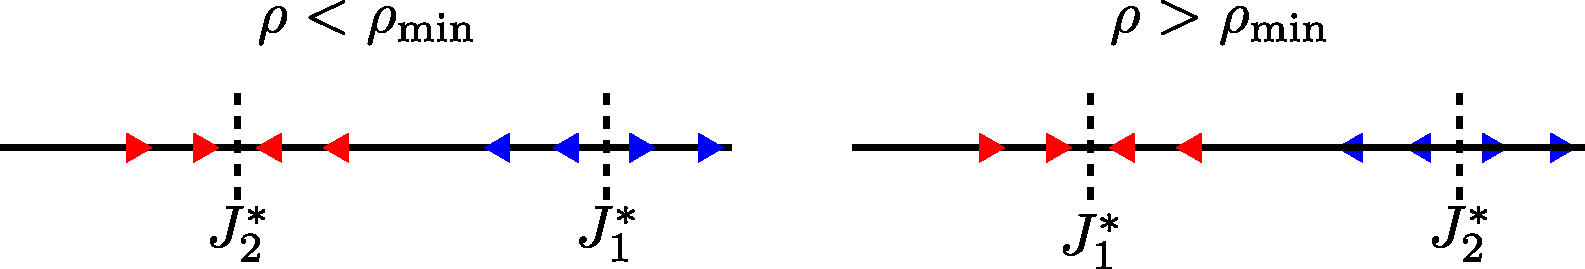
\includegraphics[width=0.45\textwidth]{./rg_flow.pdf}
	\caption{The three fixed points of the over-screened RG equation. Only the intermediate one is stable.}
	\label{rg_flow}
\end{figure}

The RG equation reduces to the perturbative form \(\Delta J_{(j)} \simeq \frac{J_{(j)}^2 \mathcal{N}_{(j)}}{D_{(j)}}\left( 1 - \frac{1}{2}\rho J_{(j)} K \right)\)~\cite{Kogan_2018,Kuramoto1998,Noz_blandin_1980,tripathi2018landau} when one replaces \(\omega_{(j)}\) with the ground state energy \(-\frac{D_{(j)}}{2}\) and assumes \(J \ll D_{(j)}\).

\subsection{Star graph as the effective fixed point Hamiltonian}
The fixed point Hamiltonian takes the form
\begin{equation}\begin{aligned}
	H^* = \sum_l\left[ \sum^*_{k}\epsilon_{k,l} \hat n_{k\alpha,l} + J\sum_{kk^\prime}^* \vec{S_d}\cdot\frac{1}{2}\vec{\sigma}_{\alpha\alpha^\prime}c_{k\alpha,l}^\dagger c_{k^\prime\alpha^\prime, l}~.\right]
\end{aligned}\end{equation}
We have not explicitly written the decoupled degrees of freedom \(D_{(j)} > D^*\) in the Hamiltonian. The \(*\) over the summations indicate that only the momenta inside the window \(D^*\) enter the summation. There is an implied summation over the spin indices \(\alpha,\beta\).

To study the low energy physics and universality of the problem, we will mostly focus on the zero bandwidth limit of the fixed point Hamiltonian. Upon setting the chemical potential equal to the Fermi energy, this zero bandwidth model becomes a Heisenberg spin-exchange Hamiltonian.
\begin{equation}\begin{aligned}
	\label{stargraph}
	H^* = J\sum_l\sum_{kk^\prime}^* \vec{S_d}\cdot\frac{1}{2}\vec{\sigma}_{\alpha\alpha^\prime}c_{k\alpha,l}^\dagger c_{k^\prime\alpha^\prime, l} = J\vec{S_d}\cdot\sum_l \vec{s}_l~.
\end{aligned}\end{equation}
At the last step, we defined the local spin operator \(\vec{s}_l = \frac{1}{2}\sigma_l = \frac{1}{2}\sum_{kk^\prime}^*\sum_{\alpha\beta}\vec{\sigma}_{\alpha\alpha^\prime}c_{k\alpha,l}^\dagger c_{k^\prime\alpha^\prime, l}\) of each conduction channel.
\begin{figure}[htpb]
	\centering
	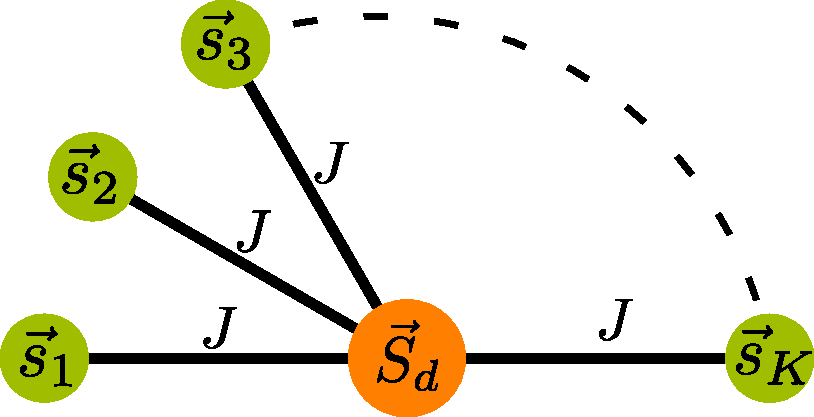
\includegraphics[width=0.45\textwidth]{./stargraph.pdf}
	\caption{Zero bandwidth limit of the fixed point Hamiltonian. The central yellow node is the impurity spin, which is talking withe the local spins of the channels represented as green nodes.}
	\label{fig:-stargraph-pdf}
\end{figure}
The star graph commutes with several operators, including the total spin operator \(J^z = S_d^z + \sum_l s_l^z\) along \(z\), the total bath local spin operator \(s^2_\text{tot} = \left(\sum_l \vec s_l\right)^2\) and the string operators 
\begin{equation}\begin{aligned}
\pi^{x,y,z} = \sigma_d^{x,y,z} \otimes_{l=1}^K \sigma_l^{x,y,z}~.
\end{aligned}\end{equation}
The \(\pi^z\) acts on the eigenstates \(\ket{J^z}\) and reveals the odd/even parity of the eigenvalue \(J^z\), and is hence a parity operator. Interestingly, the modified string operator \(\sigma_d^z \pi^z\) is a Wilson loop that wraps around the outer nodes of the star graph:
\begin{equation}\begin{aligned}
	\label{w_loop}
	\pi^z_c \equiv \sigma_d^z \pi^z = \exp\left[i \frac{\pi}{2} \left(\sum_{l=1}^K \sigma^z_l - K\right)\right] 
\end{aligned}\end{equation}
\(\pi^x\) and \(\pi^y\) mix states of opposite parity. For example, it can be shown that \(\pi^x \ket{J^z} = -\ket{J^z}\). The corresponding modified string operator \(\pi^x_c \equiv \sigma_d^x \pi^x\) is an 't Hooft operator \cite{fradkin2013field}.


There are multiple reasons for working with the star graph in particular and zero mode Hamiltonians in general. In the URG analysis of the one dimensional Hubbard model \cite{1dhubjhep}, a study of the zero mode Hamiltonian (in that case, the Fermi surface itself) was sufficient to topologically characterize various phases of the Berezinskii-Kosterlitz-Thouless (BKT) RG phase diagram. In the single-channel Kondo model, the star graph is just the two spin Heisenberg, and it shares its ground state with the full Kondo model itself~\cite{varma_yafet_1976,yosida_1966,wilson1975renormalization} along with thermodynamic properties \cite{varma_yafet_1976,kondo_urg}. Within the MCK model itself, the star graph is able to mimic the nature of the RG flows: At weak coupling \(J \to 0^+\), the central spin is weakly coupled to the outer spins and  prone to screening because of the \(s^\pm\) terms in the star graph, and at strong coupling \(J \to \infty^-\), the outer spin-half objects tightly bind with the central spin-half object to form a single spin object that interacts with the remaining states through an exchange coupling which is RG relevant, rendering both the terminal fixed points unstable. The true stable fixed point must then lie somewhere in between, and we recover the schematic phase diagram of fig.~\ref{rg_flow}. 

Our claim is that the non-Fermi liquid arises solely from the degeneracy of the ground state manifold of the underlying zero mode Hamiltonian, and the star graph captures the degeneracy in its entirety. The RG flows of the MCK model have been show to \textit{preserve the degeneracy of the ground state}~\cite{pang_cox_1991,kroha_kolf_2007,zitko_fabrizio_2017,moca_zarand_2021}\textcolor{red}. The star graph conserves the total spin \(S^z\), and this leads to a \(K-\)fold degeneracy in the ground state of the \(K-\)channel spin-half star graph which is preserved under the RG flow. This is qualitatively different from the case of the single-channel Kondo model where the \(2-\)fold degeneracy of the local moment fixed point crosses over into a stable and unique singlet ground state. 

The importance of the degeneracy can be shown in the following manner. The ground state degeneracy of the more general star graph with a spin-\(S\) impurity and \(K\) channels is given by \(g^S_K = |K - 2S|+1\). The cases of \(K=2S\), \(K<2S\) and \(K>2S\) correspond to exactly screened, under-screened and over-screened regimes respectively. The latter two cases correspond to a multiply-degenerate manifold \(g^S_K > 1\), and simultaneously have non-Fermi liquid phases~\cite{Noz_blandin_1980,Gan_Andrei_Coleman_1993,emery_kivelson,Gan_mchannel_1994,Tsvelick_Weigmann_mchannel_1984,Tsvelick_weigmann_mchannel_1985,parcollet_olivier_large_N,kimura_taro_Su_N_kondo,PhysRevB.73.224445,cox_jarrell_two_channel_rev,affleck_1991_overscreen,Coleman_tsvelik,affleck1993exact,coleman_pepin_2003,roch_nicolas_costi_2009,schiller_avraham_2008,Durganandini_2011}, while the first regime has a unique ground state \(g^S_K = 1\) and is described by a local Fermi liquid phase \cite{wilson1975,nozieres1974fermi,Noz_blandin_1980,andreiKondoreview,tsvelickKondoreview}, thereby substantiating the claim that a degeneracy greater than unity leads to non-Fermi liquid physics. The multiple ground states available to the impurity+bath system leads to a frustration of the singlet order, and we the focus of this work is to illustrate how this quantum-mechanical frustration leads to all the interesting properties of the MCK model.
\section{Important Properties of the Star Graph}
\subsection{Spectral and Quantum-mechanical features}

\subsection{Degree of compensation: a measure of the frustration}
One can quantify the amount of screening of the local moment at the impurity site by defining a degree of compensation \(\kappa\). Such a quantity also measures the inherent singlet frustration in the problem: the higher the degree of compensation, the better the spin can be screened into a singlet and lower is the frustration. It is given by the antiferromagnetic correlation existing between the impurity spin and conduction electron channels:
\begin{equation}\begin{aligned}
	\Gamma \equiv - \left< \vec{S_d}\cdot \vec{s}_\text{tot}\right>
\end{aligned}\end{equation}
where \(\vec s_\text{tot} = \sum_l \vec s_l\). The expectation value is calculated in the ground state. Since the inner product is simply the ground state energy of a spin-\(S\) impurity \(K-\)channel MCK model in units of the exchange coupling \(J\), we have
\begin{equation}\begin{aligned}
	\Gamma = \frac{1}{2} \left[ l_\text{imp}^2 + l_c^2 - g^S_K\left( g^S_K - 1 \right)\right]
\end{aligned}\end{equation}
\(l_\text{imp}^2 = S(S+1)\) is the length-squared of the impurity spin. Similarly, \(l_c^2 = \frac{K}{2}\left(\frac{K}{2} + 1\right) \) is the length-squared of the total conduction bath spin. \(g^S_K = |\frac{K}{2} - S| + 1\) is the ground state degeneracy. We will explore the three regimes of screening by defining \(K = K_0 + \delta, S = \frac{K_0}{2} - \delta\). \(\delta=0\) represents the exactly-screened case of \(K = 2S = K_0\). Non-zero \(\delta\) represents either over- or under-screening. In terms of \(K_0\) and \(\delta\), the degree of compensation becomes
\begin{equation}\begin{aligned}
	\label{gamma}
	\Gamma = \frac{1}{4}\left[\left( K_0 + 1 \right) ^2 - \left(|\delta| + 1 \right) ^2\right] 
\end{aligned}\end{equation}
For a given \(K_0\), the degree of compensation is maximised for exact screening \(\delta=0\), and is reduced for \(\delta \neq 0\). This shows the inability of the system to form a unique singlet ground state and reveals the quantum-mechanical frustration inherent in the zero mode Hamiltonian and therefore in the entire problem.
\begin{figure}[htpb]
	\centering
	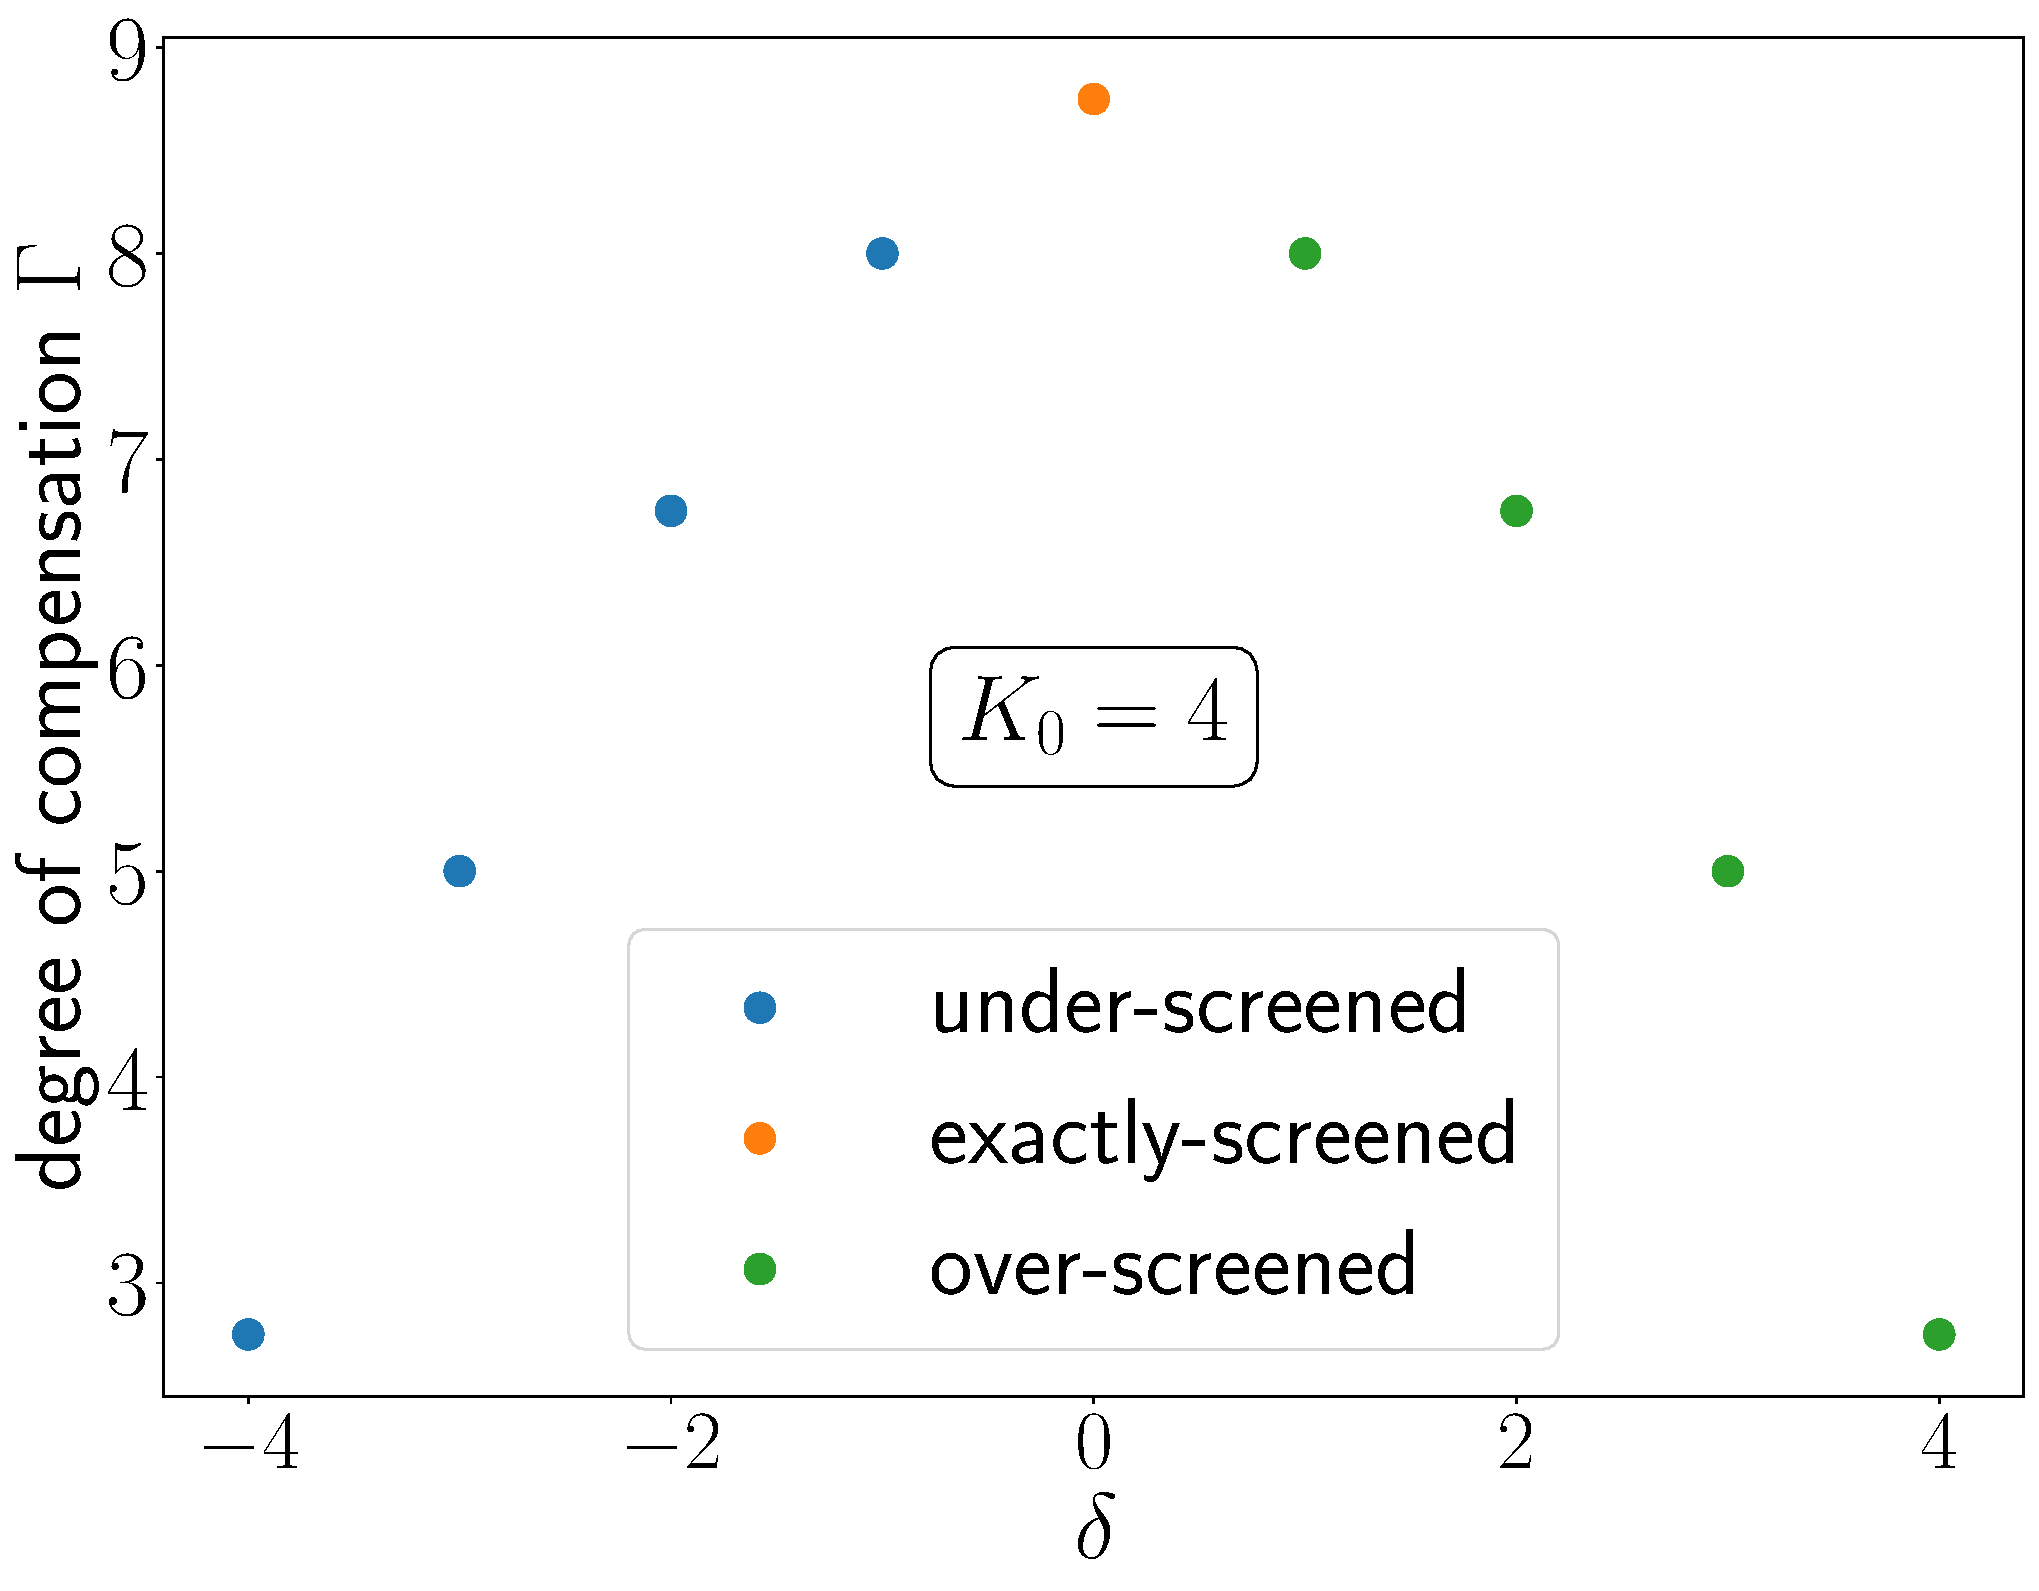
\includegraphics[width=0.45\textwidth]{../numerics/deg_of_comp.pdf}
	\caption{Variation of the degree of compensation as we tune the system from under-screening to over-screening. The maximum spin compensation occurs at exact-screening \(\delta=0\).}
\end{figure}

\subsection{Measures of entanglement}

\subsection{Twist operators and Gauge theories}

\subsection{Impurity magnetization and susceptibility: Quantum criticality of overscreened MCK model}
The channel isotropic MCK model is critical; any perturbation away from the perfectly symmetric model in terms of anisotropy is relevant, as shown in section \ref{anisotropic_rg}~\cite{vojta_2006,andrew_bulla_2011,pang_cox_1991}. This critical nature leads to several signatures that can be obtained directly from the star graph. These signatures include a discontinuity in the impurity magnetization at zero temperature in the limit of the external field going to zero, and a diverging susceptibility as temperature goes to zero.

We insert a magnetic field that acts only on the impurity and then diagonalize the Hamiltonian.
\begin{align}
	\label{stargraph_field_hamiltonian}
	H(h) = J^* \vec{S_d}\cdot\vec{s}_\text{tot} + h S_d^z
\end{align}
The Hamiltonian commutes with \(s_\text{tot}\), so it is already block-diagonal in terms of the eigenvalues \(M\) of \(s_\text{tot}\). \(M\) takes values in the range \(\left[M_\text{min}, M_\text{max}\right]\), where \(M_\text{max} = K/2\) for a \(K-\)channel Kondo model, and \(M_\text{min} = 0\)  if \(K\) is even, otherwise \(\frac{1}{2}\). Within each block, the Hamiltonian splits into independent \(2\times 2\) blocks characterized by eigenvalues of the total spin operator \(J^z = S_d^z + s^z_\text{tot}\). Defining \(\alpha = \frac{1}{2}\left(Jm + h\right) + \frac{J}{4}\) and \(x^M_m = M(M+1) - m(m+1)\), the partition function can be written as
\begin{align}
	Z(h) =\sum_{M=M_\text{min}}^{M_\text{max}}r^K_M\left[\sum_{m=-M, \atop{m\in \mathbb{Z}}}^{M-1}2e^{\beta \frac{J}{4}}\cosh \beta\sqrt{J^2x^M_m/4 + \alpha^2} \right.\nonumber\\
\left.+ 2e^{-\beta JM/2}\cosh \beta h/2\right]
\end{align}
Here, \(\beta = \frac{1}{k_B T}\), \(M\) sums over the eigenvalues of \(s_\text{tot}\) while \(m\) sums over \(J^z - \frac{1}{2}\) and the additional degeneracy factor \(r^K_M\) arises from the possibility that there are multiple subspaces defined by \(s_\text{tot}=M\). This multiplicity is given by
\begin{align}
	\label{extra_degen}
	r^K_M = {}^{K-1}C_{K/2 - M}
\end{align}

To calculate the impurity magnetic susceptibility, we will use the expression
\begin{align}
	\chi = \frac{1}{\beta}\lim_{h \to 0}\left[\frac{Z(h)^{\prime\prime}}{Z(h)} - \left(\frac{Z(h)^{\prime}}{Z(h)}\right)^2 \right] 
\end{align}
where the \(\prime\) indicates derivative with respect to \(h\). For brevity, we define \(\theta_M = \beta J (M+\frac{1}{2})/2\) and \(\Sigma_M = \sum_{m=-M, \atop{m\in \mathbb{Z}}}^{M-1}(m+\frac{1}{2})^2\). The derivatives are
\begin{align}
	\lim_{h \to 0}Z(h) &= \sum_{M=M_\text{min}}^{M_\text{max}}r^K_M\left[4Me^{\beta \frac{J}{4}}\cosh \theta_M + 2e^{-\beta JM/2}\right]\\
	\lim_{h \to 0}\frac{\:\mathrm{d}Z(h)}{\:\mathrm{d}h} &=  0\\
	\lim_{h \to 0}\frac{\:\mathrm{d}^2Z(h)}{\:\mathrm{d}h^2} &= \frac{\beta^2}{2}\sum_{M=M_\text{min}}^{M_\text{max}}r^K_M\left[\frac{e^{\beta \frac{J}{4}}}{\theta_M}\left(2M\sinh \theta_M + \right.\right.\nonumber\\
								 &\left.\left.\frac{\beta^2 J^2}{4}\left[\frac{\cosh\theta_M}{\theta_M} - \frac{\sinh \theta_M}{\theta_M^2}\right]\Sigma_M\right)+ e^{-\beta JM/2}\right]
\end{align}
At low temperature \(\beta \to \infty\), only the highest value \(M_\text{max}\) will survive:
\begin{align}
	Z &\to 2 r^K_{M_\text{max}} M_\text{max} e^{\beta \frac{J}{2}(M_\text{max} + 1)}\\
	Z^{\prime \prime} &\to r^K_{M_\text{max}}\left(\frac{\beta }{2(M_\text{max} + \frac{1}{2})}\right)^2 e^{\beta \frac{J}{2}(M_\text{max} + 1)}\Sigma_{M_\text{max}}\\
	\chi &\to \frac{\beta\Sigma_\text{max}}{2M_\text{max}\left(2M_\text{max}+1\right)^2} = \frac{\beta(K-1)}{12(K+1)} \sim \frac{1}{T}
\end{align}

This non-analyticity in a response function is a signature of the critical nature of the Hamiltonian. This is in contrast to the behaviour in the non-critical exactly-screened fixed point where the ground state is unique. There, the susceptibility becomes constant at low temperatures: \(\chi(T\to 0) = \frac{W}{4 T_K}\), \(T_K\) being the single-channel Kondo temperature and \(W\) the Wilson number \cite{wilson1975renormalization,nozieres1974fermi,bullaNRGreview,kondo_urg}. We have checked the case of general spin-\(S\) impurity numerically, and the general conclusion is that all exactly-screened models show a constant impurity susceptibility at \(T \to 0\), while the over-screened and under-screened cases show a diverging impurity susceptibility in the same limit. 

Another non-analyticity arises when we consider the impurity free energy and the magnetization. The thermal free energy is given by
\begin{equation}\begin{aligned}
	F(h) = -\frac{1}{\beta}\ln Z(h) = -\frac{1}{\beta}\ln\sum_{E_n}e^{-\beta E_n}
\end{aligned}\end{equation}
At \(T \to 0\), only the most negative energy \(E_\text{min}\) survives. Assuming a non-degenerate ground state for \(h \neq 0\), the zero temperature free energy becomes
\begin{equation}\begin{aligned}
	F(h\neq 0, T\to 0) = -\frac{1}{\beta}\ln e^{-\beta E_\text{min}} = E_\text{min}
\end{aligned}\end{equation}
In the star graph Hamiltonian with \(K-\)channels and in the presence of a field on the impurity (eq.~\ref{stargraph_field_hamiltonian}), the ground state energy will be one of the negative eigenvalues:
\begin{equation}\begin{aligned}
	\lambda^{M,h}_{m, -} = - \frac{J}{4} - \frac{1}{2}\sqrt{J^2(M+1/2)^2 + h^2 + 2hJ(m+1/2)}
\end{aligned}\end{equation}
The minimum eigenvalue is obtained by maximizing \(h(m+1/2)\). For \(h>0\), the ground state is renormalised for the most positive value of \(m\), which is \(M-1\). On the other hand, for \(h<0\), it occurs for \(m=-M\), because that is the most negative value it can take. Among all the values of \(M\), the global ground state is at the largest value of \(M\), \(K/2\). Therefore, the minimal energy eigenvalue is
\begin{equation}\begin{aligned}
	E_\text{min} = - \frac{J}{4} - \frac{1}{2}\sqrt{J^2(K+1)^2/4 + h^2 + |h|J(K-1)}
\end{aligned}\end{equation}
The first derivative of the free energy with respect to the field gives
\begin{equation}\begin{aligned}
	F^\prime(h\neq 0, T\to 0) =- \frac{2h + J(K-1)\text{sign}(h)}{4\sqrt{\frac{J^2}{4}(K+1)^2 + h^2 + |h|J(K-1)}}
\end{aligned}\end{equation}
There we used the result that the derivative of \(|x|\) is \(\text{sign}(x)\). If we now take \(h\) to zero from both directions, we get the magnetization of the impurity
\begin{equation}\begin{aligned}
	m = F^\prime(h \to 0^\pm, T\to 0) = \mp \frac{1}{2}\frac{(K-1)}{(K+1)}
\end{aligned}\end{equation}
\begin{figure}[!htpb]
	\centering
	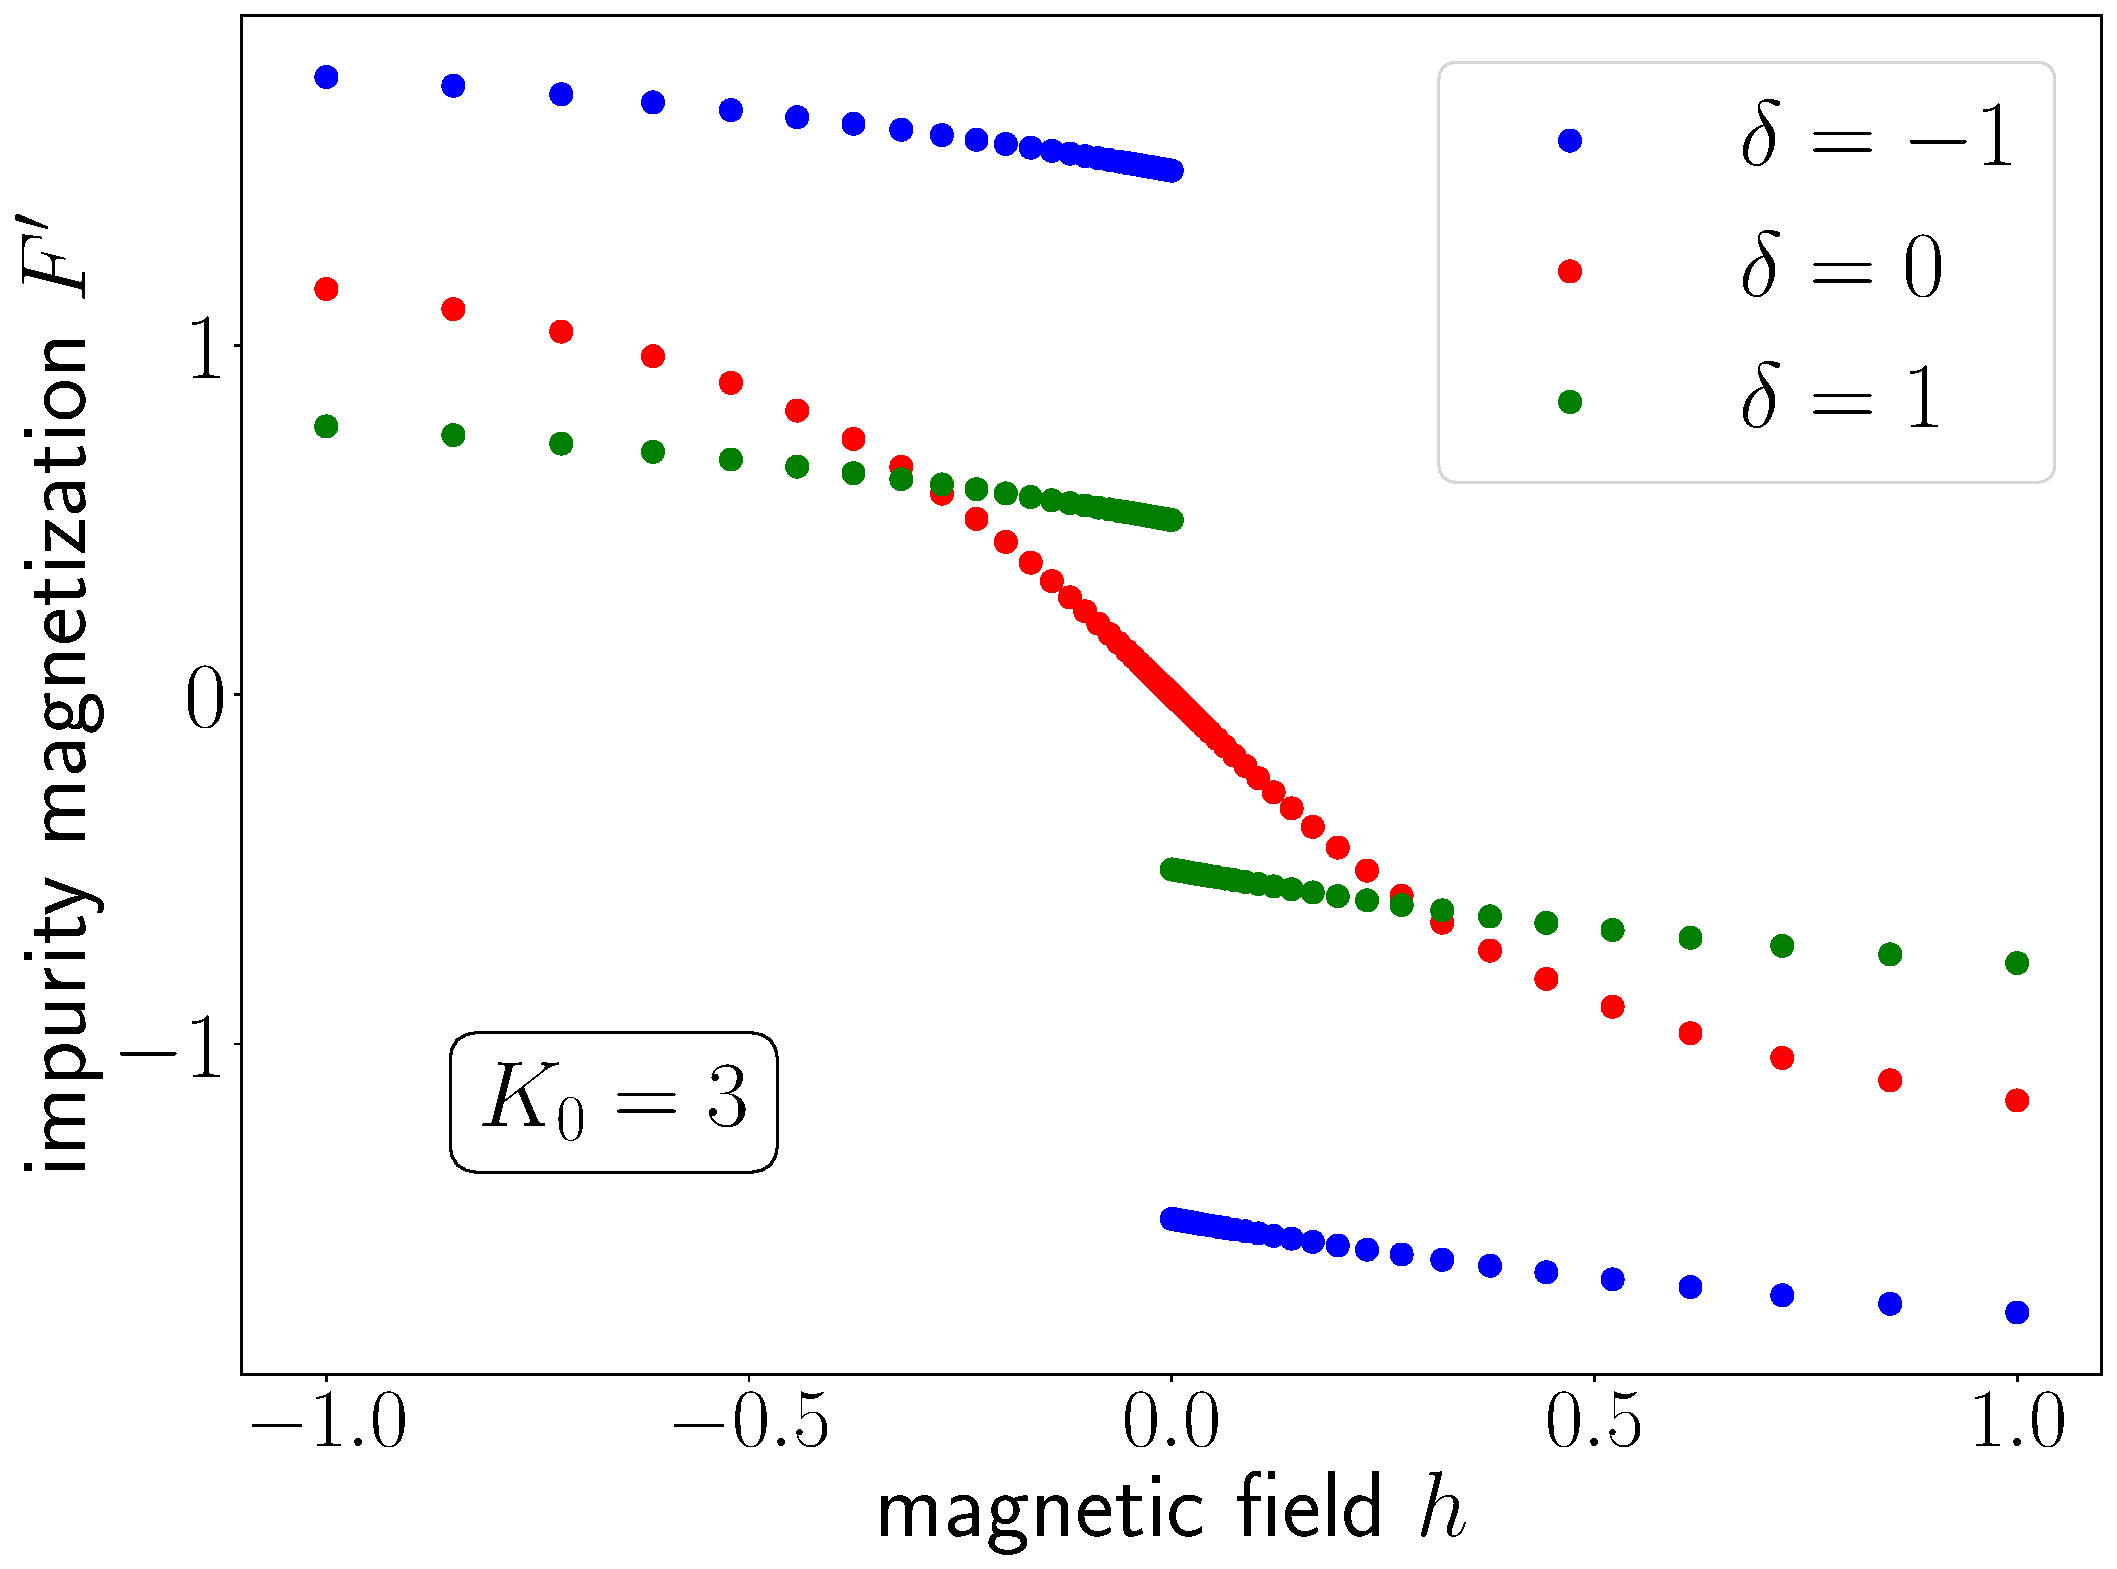
\includegraphics[width=0.45\textwidth]{../numerics/disc_mag_imp_gen.pdf}
	\caption{Behaviour of the impurity magnetization for three values of \(\left(K, 2S\right) = \left(2, 4\right), \left( 3,3 \right), \left(4, 2\right)  \). Only the case of \(K=2S=3 \left(\delta=0\right)\) is analytic near zero. The non-analyticity of the other cases arises because of the frustration brought about by the degeneracy of the star graph ground state.}
	\label{mag_crit}
\end{figure}

The magnetization is therefore discontinuous as \(h\to 0\); it goes to different values depending on the direction in which we take the limit. The non-analyticity for \(K>1\) occurs because there is at least one pair of ground state with non-zero parity \(\pi^z\) and magnetic field is able to flip one ground state into the state of opposite parity. This available space for scattering is simply the frustration that we discussed earlier. This argument, along with the diverging susceptibility for the over- and under-screened cases, makes it clear that the non-analyticity and hence the critical nature of the fixed point arise because of the ground state degeneracy, and is therefore a feature of all over-screened and under-screened  models. Indeed, we have checked numerically that the non-analyticity exists for \(\delta \neq 0\), where \(\delta = \frac{K}{2} - S\) is the deviation from exact screening. For \(\delta=0\), the ground state is unique and un-frustrated, so the external magnetic field has no parity-inverted pair to flip across.

\subsection{Impurity magnetization in terms of parity operators}
The expectation value of the impurity magnetization along a particular direction and in specific ground states can be related to the 't Hooft operator defined under eq.~\ref{w_loop}. We will work in the state comprised of two adjacent eigenstates of \(J^z\):
\begin{equation}\begin{aligned}
	\ket{g^\theta_{J^z}} \equiv \frac{1}{\sqrt 2}\left( \ket{J^z} + e^{i\theta}\ket{J^z+1}\right), && J^z < \frac{1}{2}\left( K-1 \right)
\end{aligned}\end{equation}
The expectation value of the impurity magnetization operator \(\sigma_d^x\) can be expressed as
\begin{equation}\begin{aligned}
	\left<\sigma_d^x\right> \equiv \langle g^\theta_{J^z} \vert \sigma_d^x \vert g^\theta_{J^z}\rangle = - \langle J^z + 1 \vert \pi^x_c \vert -J^z \rangle + \text{h.c.}
\end{aligned}\end{equation}
This expression relates the observable impurity magnetization to the topological 't Hooft operator \cite{Maric2020}. Evaluating the matrix elements gives
\begin{equation}\begin{aligned}
	\label{sigmax}
	\left<\sigma_d^x\right> = - \frac{\sqrt{K^2 - (2J^z + 1)^2}}{2(1+K)}\cos \theta
\end{aligned}\end{equation}
Performing a similar calculation reveals that the impurity magnetizations along \(y\) and \(z\) in the same state are given by
\begin{equation}\begin{aligned}
	\label{sigmayz}
	\left<\sigma_d^y\right> = - \frac{\sqrt{K^2 - (2J^z + 1)^2}}{2(1+K)}\sin \theta, &&\left<\sigma_d^z\right> = - \frac{2J^z + 1}{(1+K)}
\end{aligned}\end{equation}
Combining eqs.~\ref{sigmax} and \ref{sigmayz}, we find
\begin{equation}\begin{aligned}
	\cos^2\theta\left(\left<\sigma^x_d\right>\right)^2 + \sin^2\theta\left(\left<\sigma^y_d\right>\right)^2 + \frac{1}{4}\left(\left<\sigma^z_d\right>\right)^2 = \frac{1}{4}\left(\frac{K}{1+K}\right)^2
\end{aligned}\end{equation}
This relation constrains the values of the magnetization along all the directions: the \(x\) and \(y\) magnetization values have already been shown to be related to the `t Hooft operators \(\pi^x\) and \(\pi^y\) and the magnetization along \(z\) is therefore constrained in terms of the `t Hooft operators and the quantized function on the right-hand side (the function is quantized because \(K\) can only take integer values).






\section{Effect of conduction bath excitations on the fixed point theory}
\subsection{Non-Fermi liquid effective Hamiltonian}

\subsection{Presence of a marginal Fermi liquid: Orthogonality catastrophe in two-channel MCK model}
At the stable fixed point \(J ^* = J_1^* = \frac{2}{K \rho}\), the ground states of the Hamiltonian are those of the star graph model, with a degeneracy of \(K\). We now specialise to the two-channel Kondo model. To find the low-energy excitations on top of this ground state manifold, we insert a tight-binding nearest-neighbour hopping between the zeroth site (the one that holds the impurity) and the first site (site that's nearest to the zeroth site) as a perturbation and calculate the diagonal and off-diagonal terms generated by this perturbation. It is found that when we trace out the impurity, we are left only with real space off-diagonal terms:
\begin{equation}\begin{aligned}
	\label{nfl_terms}
	V_\text{eff} = \frac{2t^2}{J^*}\left[\left(\sigma^z_{0,1}\right)^2 s^+_{0,2} + \left(\sigma^z_{0,2}\right)^2 s^+_{0,1}\right] \left(s^-_{1,1} + s^-_{1,2}\right) + \text{h.c.}
\end{aligned}\end{equation}
where \(\sigma^z_{0,l} = \hat n_{0\uparrow,l} - \hat n_{0\downarrow,l}, s^+ = c^\dagger_{0 \uparrow,l}c_{0 \downarrow,l}\) and \(s^- = \left(s^+\right)^\dagger\). The notation \(0\sigma,l\) has the site index \(i=0,1,2,\ldots\) as the first label, the spin index \(\sigma=\uparrow,\downarrow\) as the second label and the channel index \(l=1,2\) as the third index.

These are the terms that are generated because of the presence of the impurity. Such a non-Fermi liquid (NFL) contribution to the effective Hamiltonian and the absence of any Fermi-liquid term at the same order should be contrasted with the local Fermi liquid excitations induced by the singlet ground state of the single-channel Kondo model~\cite{nozieres1974fermi,wilson1975renormalization,hewson1993}. We wish to point out that such NFL terms were also obtained by Coleman, et al.~\cite{Coleman_tsvelik} in terms of Majorana fermions at the zeroth site and the first site of the \(\sigma-\tau\) version of the two-channel Kondo model. They then went on to compute a single-particle self-energy renormalisation coming from this NFL term that matches the phenomenological~\cite{varma2002singular} and microscopic forms of the marginal Fermi liquid self-energy~\cite{anirbanmott1,anirbanurg1}. We take a different route in order to calculate the self-energy contribution coming from Eq.~\ref{nfl_terms}.

In the URG analysis of the 2D Hubbard model at half-filling~\cite{anirbanurg1}, it was found that the normal phase of the Mott insulator was a metal with properties that have been phenomenologically attributed to the marginal Fermi liquid. The excitations of such a phase are described by a two particle-one hole composite object:
\begin{equation}\begin{aligned}
	\label{mfl_urg}
	H_\text{MFL} = \sum_{k,k^\prime,k^{\prime\prime},\sigma}R \hat n_{k\sigma} \hat n_{k^\prime \overline\sigma}\left(1 - \hat n_{k^{\prime\prime}\sigma}\right) 
\end{aligned}\end{equation}
We wish to look for such a term in the effective Hamiltonian. For this, we will perform a perturbative treatment of the hopping at strong coupling \(J \to \infty\) where the perturbative coupling \(t^2/J\) is arbitrarily small and again obtain Eq.~\ref{nfl_terms}. Such a change from the strong coupling model with parameter \(J\) to a weak coupling model with parameter \(t^2/J\) amounts to a duality transformation~\cite{kroha_kolf_2007,zitko_fabrizio_2017}. It can be shown that the duality transformation leads to an identical MCK model~\cite{kroha_kolf_2007} (self-duality), which implies we can have identical RG flows, and our transformation simply extracts the NFL piece from the dual model. The self-duality also ensures that the critical intermediate-coupling fixed point is unique and can be reached from either of the models.

The diagonal part of eq.~\ref{nfl_terms} is
\begin{equation}\begin{aligned}
	V_\text{eff} = \frac{2t^2}{J}\sum_{l=1,2}\left(\sum_\sigma \hat n_{0\sigma,l}\right) s^+_{0,\bar l}s^-_{1,\bar l} + \text{h.c.}
\end{aligned}\end{equation}
where \(\bar l = 3 - l\) is the channel index complementary to \(l\). We will fourier transform this effective Hamiltonian into \(k-\)space. The NFL part becomes
\begin{equation}\begin{aligned}
	\label{k_space_od}
	\sum_{\sigma, \left\{k_i,k_i^\prime\right\},l} \frac{2t^2}{J}e^{i\left(k_1 - k_1^\prime\right)a}c^\dagger_{k\sigma,l}c_{k^\prime\sigma,l}c^\dagger_{k_2 \uparrow, \bar l}c_{k_2^\prime \downarrow,\bar l}c^\dagger_{k_1 \downarrow,\bar l}c_{k_1^\prime \uparrow, \bar l} + \text{h.c.} 
\end{aligned}\end{equation}
This form of the Hamiltonian is very similar to the three-particle interaction term in Appendix B of~\cite{anirbanmott1}. The channel indices in Eq.~\ref{k_space_od} can be mapped to the normal directions in~\cite{anirbanmott1}. As specualted eariler, the 2 particle-1 hole interaction in Eq.~\ref{k_space_od} has a diagonal component which can be obtained by setting \(k=k^\prime, k_1 = k_2^\prime\) and \(k_2 = k_1^\prime\):
\begin{equation}\begin{aligned}
	H_\text{eff,MFL} = \sum_{k, k_1, \atop{k_2,\sigma,  l}} \frac{2t^2e^{i\left(k_1 - k_2\right)a}}{J} \hat n_{k\sigma,l} \hat n_{k_2 \uparrow, \bar l}\left(1 - \hat n_{k_1 \downarrow,\bar l}\right) + \text{h.c.}\\
	= \sum_{k, k_1, \atop{k_2,\sigma,  l}} \frac{4t^2}{J} \cos a\left(k_1 - k_2\right)  \hat n_{k\sigma,l} \hat n_{k_2 \uparrow, \bar l}\left(1 - \hat n_{k_1 \downarrow,\bar l}\right)
\end{aligned}\end{equation}
The most dominant contribution comes from \(k_1 = k_2 = k^\prime\), revealing the non-Fermi liquid metal~\cite{cox_jarrell_two_channel_rev,andrei_jerez_1995}:
\begin{equation}\begin{aligned}
	\label{mfl_large}
	H^*_\text{eff,MFL} = \frac{4t^2}{J} \sum_{\sigma, k, k^\prime, l} \hat n_{k\sigma,l} \hat n_{k^\prime \uparrow, \bar l}\left(1 - \hat n_{k^\prime \downarrow,\bar l}\right)
\end{aligned}\end{equation}
Following~\cite{anirbanmott1}, one can follow the RG evolution of the dual coupling \(R_j = \frac{4t^2}{J_j}\) at the \(j^\text{rh}\) RG step, in the form of the URG equation
\begin{equation}\begin{aligned}
	\Delta R_j =- \frac{R_j^2}{\omega - \epsilon_{j}/2 - R_j/8}
\end{aligned}\end{equation}
In the RG equation, \(\epsilon_{j}\) represents the energy of the \(j^\text{th}\) isoenergetic shell. It is seen from the RG equation that \(R\) is relevant in the range of \(\omega < \frac{1}{2}\epsilon_j\) that has been used throughout, leading to a fixed-point at \(R^*/8 = \omega - \frac{1}{2}\epsilon^*)\). The relevance of \(R\) is expected because the strong coupling \(J\) is irrelevant and \(R \sim 1/J\).

The renormalisation in \(R\) leads to a renormalisation in the single-particle self-energy~\cite{anirbanmott1}. The \(k-\)space-averaged self-energy renormalisation is
\begin{equation}\begin{aligned}
	\Delta \Sigma(\omega) = \rho {R^*}^2\int_0^{\epsilon^*} \frac{d\epsilon_j}{\omega - \epsilon_j/2 + R_j/8}
\end{aligned}\end{equation}
The density of states can be approximated to be \(N^*/R^*\), where \(N^*\) is the total number of states over the interval \(R^*\). As suggested by the fixed point value of \(R_j\), we can approximate its behaviour near the fixed point by a linear dependence of the dispersion \(\epsilon_j\). The two limits of the integration are the start and end points of the RG. We start the RG very close to the Fermi surface and move towards the fixed point \(\epsilon^*\). Near the start point, we substitute \(\epsilon = 0\) and \(R = \omega\), following the fixed point condition. From the the fixed point condition, we also substitute \(R^*/8 = \omega - \frac{1}{2}\epsilon^*\). On defining \(\bar \omega = N^* \left(\omega - \frac{1}{2}\epsilon^*\right)\), we can write
\begin{equation}\begin{aligned}
	\label{self_energy}
	\Delta \Sigma(\omega) \sim  \bar \omega \ln \frac{N^* \omega}{\bar \omega}
\end{aligned}\end{equation}
The self-energy also provides the quasiparticle residue for each channel\cite{anirbanmott1}:
\begin{equation}\begin{aligned}
	Z(\bar\omega) = \left(2 - \ln \frac{2\bar\omega}{N^* \omega}\right) ^{-1}
\end{aligned}\end{equation}
As the energy scale \(\omega \to 0\), the \(Z\) vanishes, implying that the ground state and lowest-lying excitations, in the presence of the NFL terms, are not adiabatically connected to the Fermi gas. This is the orthogonality catastrophe~\cite{varma2002singular,anderson_infraredcat,yamada_catastrophe,yamada1979orthogonality} in the two-channel Kondo problem, and it is brought about by the presence of the terms in Eq.~\ref{mfl_large}. Such terms were absent in the single-channel Kondo model, because there was no multiply-degenerate ground state manifold that allowed scattering. This line of argument shows that the extra degeneracy of the ground state subspace and the frustration of the singlet order that comes about when one upgrades from the single-channel Kondo model to the MCK models is at the heart of the NFL behaviour, and the orthogonality catastrophe should be a general feature of all such frustrated MCK models, even though we have demonstrated this only for the two-channel case. A local NFL term with a self-energy of the form in eq.~\ref{self_energy} was also obtained in the \(\sigma-\tau\) model by Coleman et al.~\cite{Coleman_tsvelik}. The common features show the universality between the two-channel Kondo and the \(\sigma-\tau\) models.
\subsection{Low temperature thermodynamic behaviour}

\subsection{Non-Fermi liquid signatures in momentum space}
Obtaining the effective Hamiltonian involves obtaining the low energy excitations on top of the ground state of the star graph. The large-energy excitations are ones that involve spin flips. This guides the separation of the Hamiltonian into a diagonal and an off-diagonal piece:
\begin{align}
	H = H_d + V = \underbrace{H_0 + J S_d^z s_\text{tot}^z}_{H_d} + \underbrace{\frac{J}{2}S_d^+ s_\text{tot}^- + \text{h.c.}}_{V + V^\dagger}
\end{align}
We define \(V\) as the interaction term that decreases \(s_\text{tot}^z\) by 1: \(V \ket{s_\text{tot}^z} \to \ket{s_\text{tot}^z - 1}\). Similarly, we define \(V^\dagger \ket{s_\text{tot}^z} \to \ket{s_\text{tot}^z + 1}\). The effective Hamiltonian that has the states \(\ket{S_d^z, s_\text{tot}, s_\text{tot}^z}\) as eigenstates are
\begin{widetext}
\begin{align}
	H_\text{eff} = H_d + V \frac{1}{E_\text{gs} - H_d}V = H_d + \frac{J}{2}S_d^+ s_\text{tot}^- \frac{1}{E_\text{gs} - J S_d^z s_\text{tot}^z - H_0}\frac{J}{2}S_d^- s_\text{tot}^+ +\frac{J}{2}S_d^- s_\text{tot}^+ \frac{1}{E_\text{gs} - J S_d^z s_\text{tot}^z - H_0}\frac{J}{2}S_d^+ s_\text{tot}^-
\end{align}
This is obtained from the Schrodinger equation for the ground state. If we expand the ground state in terms of \(\ket{S_d^z, s_\text{tot}, s_\text{tot}^z}\), we have  \(\ket{\Psi_\text{gs}} = \sum_{S_d^z, s_\text{tot},s_\text{tot}^z}C_{S_d^z, s_\text{tot},s_\text{tot}^z}\ket{S_d^z, s_\text{tot}, s_\text{tot}^z}\). The Schrodinger equation for the ground state can be written as
\begin{align}
	E_\text{gs}\ket{\Psi_\text{gs}} = H \ket{\Psi_\text{gs}} = \left(H_d + V\right)\ket{\Psi_\text{gs}} \implies \left(E_\text{gs} - H_d\right)\sum C_{S_d^z, s_\text{tot},s_\text{tot}^z}\ket{S_d^z, s_\text{tot}, s_\text{tot}^z} = V\sum C_{S_d^z, s_\text{tot},s_\text{tot}^z}\ket{S_d^z, s_\text{tot}, s_\text{tot}^z}
\end{align}
\end{widetext}
\(E_\text{gs}\) is the ground state energy, and can be replaced by the star graph ground state energy if we remove the kinetic energy cost via normal ordering: \(E_\text{gs} = -\frac{J}{2}\left(\frac{K}{2}+1\right) \). Since the interaction part \(V\) only changes \(S_d^z \to -S_d^z\) and \(s^z_\text{tot} \to s^z_\text{tot} \pm 1\), we can simplify the equation into individual smaller equations. For the two-channel model, the possible states are \((s_\text{tot},s^z_\text{tot}) = (0,0), (1,-1), (1,0), (1,1)\). The individual equations for these states are
\begin{align}
	\label{eff_ham_Sdz_10}
	E_\text{gs} \ket{\frac{1}{2}, 1, 0} &= \left(H_d + V \frac{1}{E_\text{gs} - H_d}V^\dagger\right) \ket{\frac{1}{2}, 1, 0}\\
	E_\text{gs} \ket{-\frac{1}{2}, 1, 0} &= \left(H_d + V^\dagger \frac{1}{E_\text{gs} - H_d} V\right) \ket{-\frac{1}{2}, 1, 0}\\
\end{align}
These equations represent the Schrodinger equation for the states \(\ket{S_d^z, 1, 0}\), and the right hand sides therefore give the effective Hamiltonians for those states. If we combine the states into a single subspace \(\ket{1,0}= \left\{\ket{\frac{1}{2}, 1, 0}, \ket{-\frac{1}{2}, 1, 0}\right\}\), the effective Hamiltonian for this composite subspace becomes the sum of the two parts:
\begin{align}
	\label{eff_ham_10}
	H^{1,0}_\text{eff}\ket{1, 0}\bra{1, 0} = \left(H_d + V G_0 V^\dagger + V^\dagger G_0  V\right) \ket{1, 0}
\end{align}
where \(G_0 = \left(E_\text{gs} - H_d\right)^{-1}\). If we expand the subspace as \(\ket{1,0} = \ket{\frac{1}{2}, 1, 0} + \ket{-\frac{1}{2}, 1, 0}\), we recover eqs.~\ref{eff_ham_Sdz_10}. Solving similarly for the other states gives
\begin{align}
	H^{1,1}_\text{eff}\ket{1,  1}\bra{1,  1} &= \left(H_d + V^\dagger G_0  V\right) \ket{1,  1}\\
	H^{1,-1}_\text{eff}\ket{1, - 1}\bra{1, - 1} &= \left(H_d + V G_0 V^\dagger\right) \ket{1, - 1}
\end{align}

To calculate these effective Hamiltonians, we will calculate the individual terms. We can easily simplify the \(S_d^z\) in the denominator of \(G_0\), because \(S_d^\pm \frac{1}{A + B S_d^z} = S_d^\pm \frac{1}{A \mp \frac{1}{2}B}\):
\begin{align}
	V G_0 V^\dagger = \frac{J^2}{4} s_\text{tot}^- \frac{\frac{1}{2} + S_d^z}{E_\text{gs} + \frac{J}{2} s_\text{tot}^z - H_0} s_\text{tot}^+ \\
	V^\dagger G_0 V = \frac{J^2}{4} s_\text{tot}^+ \frac{\frac{1}{2} - S_d^z}{E_\text{gs} - \frac{J}{2} s_\text{tot}^z - H_0} s_\text{tot}^-
\end{align}
Since \(H_0\) does not commute with the spin operators, we will need to expand the denominator to make sense of this Hamiltonian.
\begin{widetext}
\begin{align}
	 V G_0 V^\dagger =  s_\text{tot}^- \frac{1}{E_\text{gs} + \frac{J}{2} s_\text{tot}^z}\left[1 + \frac{1}{E_\text{gs} + \frac{J}{2} s_\text{tot}^z}H_0 + \frac{1}{E_\text{gs} + \frac{J}{2} s_\text{tot}^z}H_0\frac{1}{E_\text{gs} + \frac{J}{2} s_\text{tot}^z}H_0 + \ldots\right] s_\text{tot}^+\\
	 V^\dagger G_0 V =  s_\text{tot}^+ \frac{1}{E_\text{gs} - \frac{J}{2} s_\text{tot}^z}\left[1 + \frac{1}{E_\text{gs} - \frac{J}{2} s_\text{tot}^z}H_0 + \frac{1}{E_\text{gs} - \frac{J}{2} s_\text{tot}^z}H_0\frac{1}{E_\text{gs} - \frac{J}{2} s_\text{tot}^z}H_0 + \ldots\right] s_\text{tot}^-
\end{align}
\end{widetext}
This is an expansion in \(H_0^n/J^{n+1}, n=0,1,2,\ldots\). Expanding up to \(n=2\) and keeping at most two particle interaction terms, 
the effective Hamiltonians for these states are:
\begin{widetext}
\begin{align}
	H_\text{eff}^{1, 1} &= H_0 + J S_d^z + \frac{J^2}{4}\frac{2}{E_\text{gs}}\left[1 + \frac{H_0}{E_\text{gs}} + \frac{s^+_\text{tot}X_{1,\text{tot}}}{2 E_\text{gs}} + \frac{H_0^2 }{E_\text{gs}^2} - \frac{Z_{1,\text{tot}} H_0}{E_\text{gs}^3}\right] \left(\frac{1}{2} - S_d^z\right) \\
	H_\text{eff}^{1, -1} &= H_0 - J S_d^z + \frac{J^2}{4}\frac{2}{E_\text{gs}}\left[1 + \frac{H_0}{E_\text{gs}}  - \frac{s^-_\text{tot}X^\dagger_{1,\text{tot}}}{2 E_\text{gs}}  + \frac{H_0^2}{E_\text{gs}^2}  - \frac{ Z_{1,\text{tot}} H_0}{E_\text{gs}^3}\right] \left(\frac{1}{2} + S_d^z\right) \\
	H_\text{eff}^{1, 0} &= H_0 + \frac{J^2}{2\left(E_\text{gs} + \frac{J}{2}\right)}\left[1 + \frac{ H_0 + \left(\frac{1}{2} + S_d^z\right) s^+_\text{tot}X_{1,\text{tot}} - \left(\frac{1}{2} - S_d^z\right) s^-_\text{tot}X^\dagger_{1,\text{tot}}}{2 \left(E_\text{gs} + \frac{J}{2}\right)} + \frac{H_0^2}{\left(E_\text{gs} + \frac{J}{2}\right)^2} - \frac{Z_{1,\text{tot}} H_0}{\left(E_\text{gs} + \frac{J}{2}\right)^3} \right]
\end{align}
\end{widetext}
We employed the definitions \(X_{n,\text{tot}} \equiv  \sum_l \sum_{k,k^\prime}\left(\epsilon_k - \epsilon_{k^\prime}\right)^n c^\dagger_{k \downarrow}c_{k^\prime \uparrow},  X_{n,l}\) and \( Z_{1,\text{tot}} \equiv \sum_{k,k^\prime,l}\left( \epsilon_k - \epsilon_{k^\prime} \right) \frac{1}{2}\left(c^\dagger_{k \uparrow,l}c_{k^\prime \uparrow,l} - c^\dagger_{k \downarrow,l}c_{k^\prime \downarrow,l}\right)\). Focusing on the effective Hamiltonian for \(\left( 1,0 \right) \), we see lots of non-Fermi liquid terms of the form \(s^+_\text{tot}X_{1,\text{tot}}, s^-_\text{tot}X^\dagger_{1,\text{tot}},Z_{1,\text{tot}} H_0\). These arise because of the degenerate manifold and the increased availability of states in the Hilbert space for scattering, as compared to the unique singlet ground state of the single-channel Kondo model.


\section{Strong-weak duality of the general spin-\(S\) impurity multi-channel Kondo model}
We start from a strong coupling \((J \to \infty)\) spin-\(S\) impurity MCK Hamiltonian in the over-screened regime \(\left( K > 2S \right) \),
\begin{equation}\begin{aligned}
	\label{strong_ham}
	H(J) = \sum_{k,\sigma,l}\epsilon_{k,l} \hat n_{k\sigma,l} + J \vec{S_d}\cdot\vec{s}_\text{tot}~.
\end{aligned}\end{equation}
Here, \(\vec s_\text{tot}\) is the total spin \(\sum_l \sum_{kk^\prime \alpha\beta} \vec \sigma_{\alpha\beta}c^\dagger_{k\alpha,l}c_{k^\prime\beta,l}\) of all the zero modes. At strong-coupling, the ground states of the star graph eq.~\ref{stargraph} act as a good starting point for a perturbative expansion. As argued previously, there are \(K-2S+1\) ground states, labeled by the \(K\) values of the total spin angular momentum \(S^z = S_d^z + s_\text{tot}^z = -\frac{K}{2} + S, -\frac{K}{2} + S + 1, \ldots, \frac{K}{2} - S\). To leverage the large coupling, one can define a new spin impurity \(\mathbb{S}\) out of this ground state manifold. Since the degeneracy of a spin is given by its multiplicity \(2S^\prime + 1\), we have \(2S^\prime + 1 = K-2S+1 \implies S^\prime = \frac{K}{2} - S\). That is, the spin-\(S\) impurity has a dual described by a spin-\((K-2S+1)\) impurity. The states of this new spin are defined by
\begin{gather}
	\mathbb{S}_d^z \ket{S^z} = S^z \ket{S^z},\nonumber\\
	\mathbb{S}_d^\pm \ket{S^z} = \sqrt{S^\prime\left( S^\prime + 1 \right) - S^z\left( S^z \pm 1\right)} \ket{S^z \pm 1}
\end{gather}
The excited states of the star graph can be used to define bosons \cite{kroha_kolf_2007}, and the hopping into the lattice can then be re-written using these Bosons. One can then remove the single-particle hoping between the zero modes and the first sites using a Schrieffer-Wolff transformation in the small coupling \(J^\prime = \gamma \frac{4t^2}{J}\), and generate an exchange-coupling between the new impurity \(\vec {\mathbb{S}}_d\) and the new zero modes formed out of the remaining sites in the lattice \cite{kroha_kolf_2007} (by remaining, we mean those real space sites that have not been consumed into forming the new spin). The new Hamiltonian, characterized by the small super-exchange  coupling \(J^\prime\), has the form
\begin{equation}\begin{aligned}
	H^\prime(J^\prime) = \sum_{k,\sigma,l}\epsilon_{k,l} \hat n_{k\sigma,l} + J^\prime \vec{\mathbb{S}_d}\cdot\vec{s^\prime}_\text{tot}
\end{aligned}\end{equation}
The prime on \(s_\text{tot}\) indicates that it is formed by the new zero modes. This Hamiltonian is very similar to the one in eq.~\ref{strong_ham}, and that is the essence of the strong-weak duality: One can go from the over-screened strong coupling spin-\(S\) MCK model to another over-screened weak coupling spin-\((K-2S+1)\) MCK model. For the case of \(K=4S\), we have \(S^\prime = S\), and both \(S_d\) and \(\mathbb{S}_d\) describe the same spin objects (at least formally). The two models are then said to be self-dual. For example, for the case of spin-half MCK model, two-channel model is self-dual.
\begin{figure}[!htpb]
	\centering
	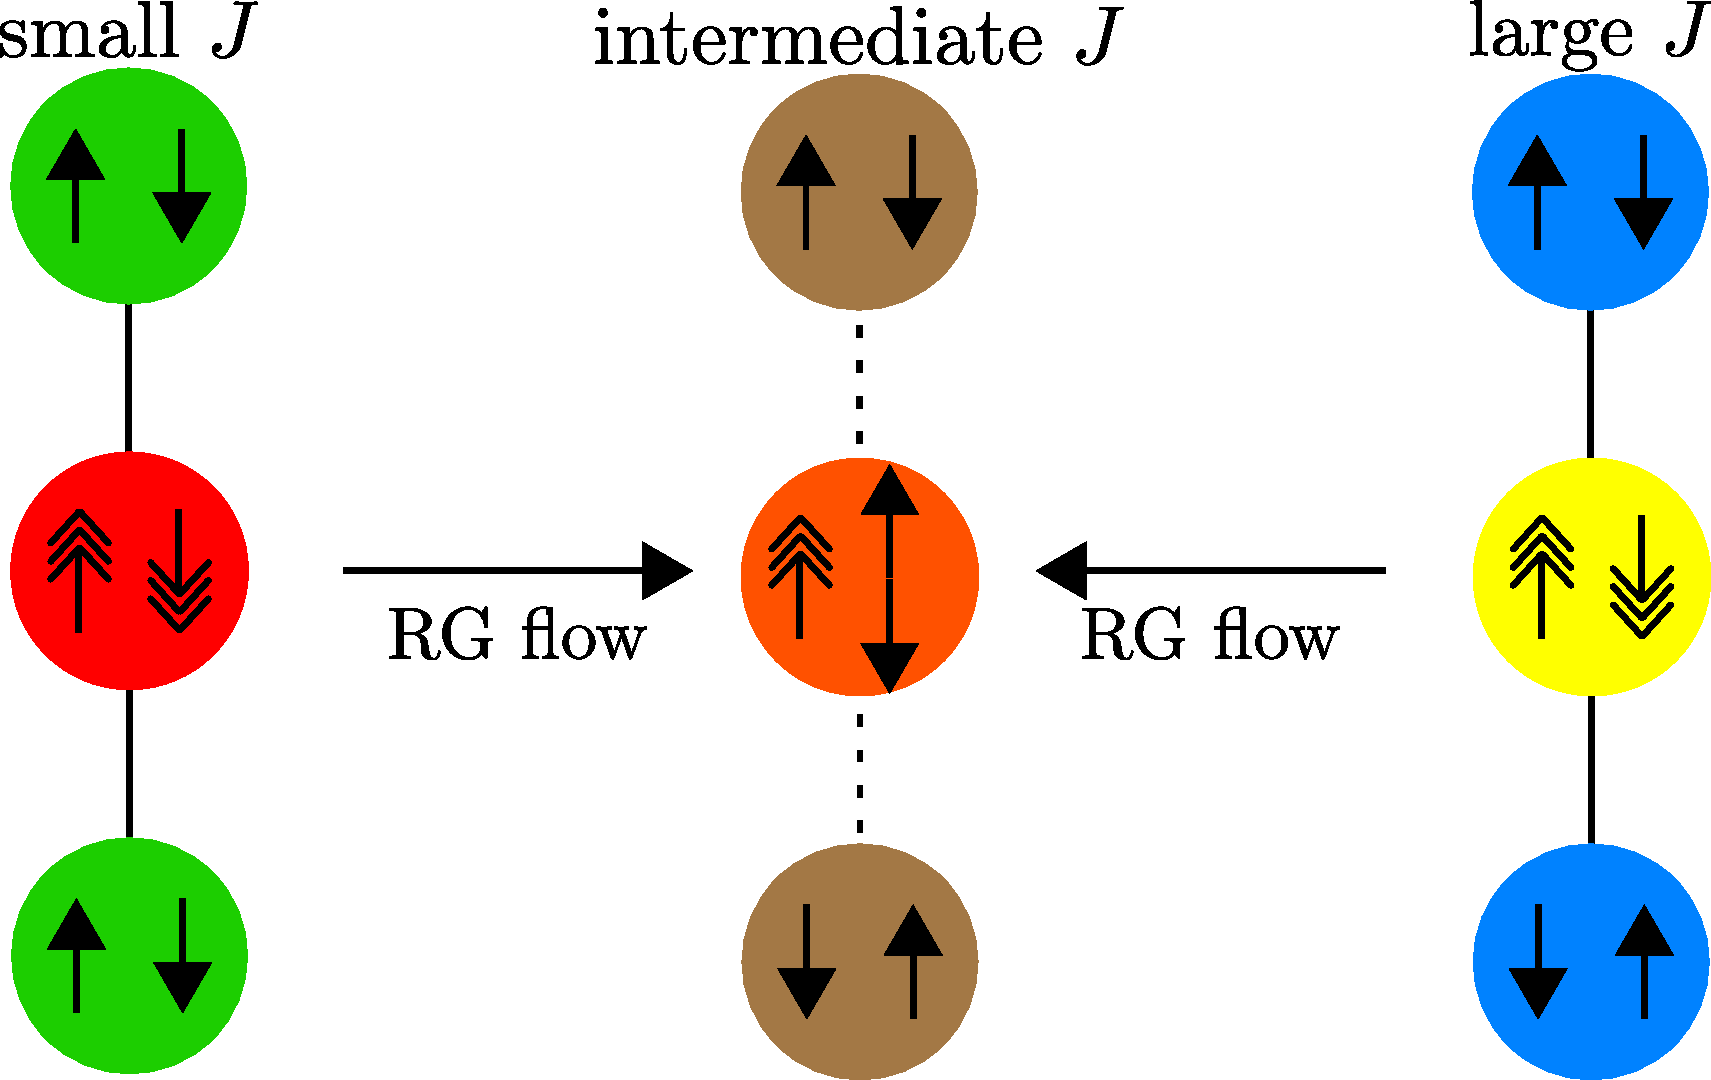
\includegraphics[width=0.4\textwidth]{./duality.pdf}
	\caption{Duality of the RG flows as seen in the star graph Hamiltonian. The red and green circles represent the impurity and zeroth site spins respectively. At large \(J\), the red circle binds with the green circles to form an effective spin \(\frac{K-1}{2}\) object (yellow) that interacts with the remaining spin of the conduction bath (blue circles).}
	\label{duality_fig}
\end{figure}

One important consequence of the duality relationship between the two over-screened models is that the RG equations are also dual; while the strong coupling model has an irrelevant coupling \(J\) that flows down to the intermediate fixed point \(J^*\), the weak coupling model has a relevant coupling \(J^\prime\) that flows up to the same fixed point \({J^\prime}^* = J^*\). From the RG equation for the general spin-\(S\) MCK model, we know that \({J^\prime}^* = \frac{2}{K \rho^\prime}\), where \(\rho^\prime\) is the DOS for the bath of the weak coupling Hamiltonian. This constrains the form of the scaling factor \(\gamma\):
\begin{equation}\begin{aligned}
	{J^\prime}^* = \frac{\gamma 4t^2}{J^*} = \frac{2}{K \rho^\prime} \implies \gamma = \frac{1}{4t^2} {J^*}^2 = \frac{1}{K^2 t^2 \rho \rho^\prime}
\end{aligned}\end{equation}

There exists another set of cross-dual points in the MCK model. This was hinted at when we looked at the degree of compassion in eq.~\ref{gamma}. Since \(\Gamma\) depends only on the magnitude of \(\delta\), both \(\pm \delta\) will give the same degree of compensation, same ground state energy and same degeneracy \(\left(g^S_K = |\delta|+1\right)\). The definition of \(\delta\)gives the duality transformation as \(K \to 2S, S \to \frac{K}{2}\). The duality therefore exists between a spin-\(S\) impurity \(K-\)channel model and a spin-\(\frac{K}{2}\) impurity \(2S-\)channel model. The exactly-screened Hamiltonian \(K=2S\) maps on to itself and is therefore self-dual under this transformation.



\section{Impurity Quantum Phase transition in the multi-channel Kondo model under channel anisotropy}
\label{anisotropic_rg}
The isotropic MCK mode undergoes a phase transition when the symmetry of the channel interaction strengths is destroyed. We will now summarize the conclusions of this section. It will be shown analytically that if, in a \(K-\)channel model, one of the couplings becomes slightly larger than the other \(K-1\) couplings, the system goes into the singlet ground state characterized by local Fermi liquid excitations. On the other hand, if one of the couplings becomes slightly smaller than the rest, the system goes over to the \(K-1\) channel Kondo model. This shows that in the context of the general anisotropic MCK model, the symmetric model is highly unstable under slight anisotropy, and undergoes a phase transition into either the \(K-1\) channel model or into the singlet ground state.
\begin{figure}[htpb]
	\centering
	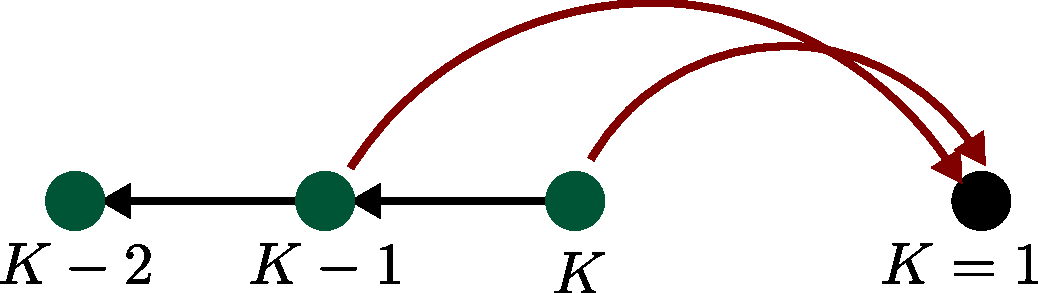
\includegraphics[width=0.4\textwidth]{./iqpt.pdf}
	\caption{Transitions from one Kondo model to another under insertion of anisotropy. The green circles represents MCK models with \(K>1\) while the black circle represents the \(K=1\) model. The red lines indicate transition from the \(K\) channel MCK model to the single-channel model when one of the exchange couplings becomes larger than the others. The black lines indicate the transition from the \(K\) channel model to the \(K-1\) channel model when one of the exchange couplings becomes smaller than the others.}
	\label{fig:-iqpt-pdf}
\end{figure}

To see the transition, we need to start with the more general anisotropic MCK model:
\begin{align}
	H = \sum_{k,\alpha,l}\epsilon_{k,l} \hat n_{k\alpha,l} + \sum_{kk^\prime,\atop{\alpha,\beta,l}}J_l \vec{S_d}\cdot\frac{1}{2}\vec{\sigma}_{\alpha\beta}c_{k\alpha,l}^\dagger c_{k^\prime\beta, l}~.
\end{align}
We now consider the specific case where \(K-1\) channels have the same coupling \(J_1 = J_2 = ... = J_{K-1} = J_+\) and the remaining channel has a different coupling \(J_K = J_-\). The RG equations for such a model are
\begin{align}
	\frac{\Delta J_\pm}{|\Delta D|} = -\frac{J_\pm^2 \rho}{\mathcal{D}_\pm} + \frac{\rho^2 J_\pm}{2}\left[\frac{(K-1)J_+^2}{\mathcal{D}_+} + \frac{J_-^2}{\mathcal{D}_-}\right]
\end{align}
where \(\mathcal{D}_\pm = \omega - \frac{D}{2} - \frac{J_\pm}{4}\) are the denominators of the URG equations.
Setting \(J_+ = J_-\) leads to the critical fixed point at \(J_+^* = J_-^* = J_* = \frac{2}{K \rho}\). We now perturb around this fixed point by defining new variables \(j_\pm = J_\pm - J_*\). We also assume that the bandwidth is large enough so that \(\mathcal{D}_\pm \simeq \omega - \frac{D}{2} - \frac{J_*}{4} = -|\mathcal{D}_*|\). The RG equations then take the form
\begin{widetext}
\begin{align}
	\frac{\Delta j_+}{|\Delta D|} &= \frac{\rho J_+}{ |\mathcal{D}_*|}\left[J_+ - \frac{\rho}{2}\left[(K-1)J_+^2 + J_-^2\right]\right] = \frac{\rho J_+}{K J_*|\mathcal{D}_*|}\left[-\left(K - 2\right)J_*j_+ - (K-1)j_+^2 - j_-^2 - 2J_* j_-\right]\\
	\frac{\Delta j_-}{|\Delta D|} &= \frac{J_- \rho}{|\mathcal{D}_*|}\left[J_- - \frac{\rho}{2}\left[(K-1)J_+^2 + J_-^2\right]\right] = \frac{J_- \rho}{K J_*|\mathcal{D}_*|}\left[\left(K - 2\right)J_*j_-  - j_-^2 - (K-1)j_+^2 - 2(K-1)J_* j_+\right]\\
\end{align}
\end{widetext}
We will first look at the special case of \(K=2\), the two channel Kondo model. The equations simplify to
\begin{align}
	\frac{\Delta j_\pm}{|\Delta D|} = \frac{J_\pm \rho}{K J_*|\mathcal{D}_*|}\left[- \left(j_+^2 + j_-^2\right) - 2J_* j_\mp\right]
\end{align}
For \(j_- < 0, j_+ > 0\), we have \(\Delta j_- < 0\). The coupling \(J_-\) therefore becomes irrelevant. For small \(j_+\), we have \(j_+^2 < 2J_* |j_-|\)  and \(\Delta j_+ > 0\). This means that the isotropic fixed point is repulsive under anisotropy~\cite{Noz_blandin_1980}. The coupling \(j_+\) being relevant means we have a single-channel Kondo problem. We already know the non-perturbative URG equation for the single-channel Kondo problem~\cite{kondo_urg}, and it leads to the strong coupling fixed point~\cite{Noz_blandin_1980,fabrizio_nozieres_1995,mitchell_bulla_2014}.

We now look at the general \(K\) channel case. Let us first look at the regime \(j_- < 0, j_+ > 0\). In this regime, we have \(\Delta j_- < 0\), which means \(j_-\) will flow to larger negative values until it reaches \(j_- = -J_*\) such that \(J_- = J_* + j_- = 0\). \(j_+\) is, on the other hand, relevant for small values of \(j_\pm\). It will continue to grow until the numerator of \(\Delta j_+\) vanishes. This condition is given by
\begin{align}
	\left(K - 2\right)J_*j_+ + (K-1)j_+^2 + j_-^2 + 2J_* j_- = 0
\end{align}
Substituting \(j_- = -J_*\) gives the fixed-point equation \((K-1)j_+^2 + \left(K - 2\right)J_*j_+ - J_*^2 = 0\). Solving the equation gives
\begin{align}
	j_{+,*} = \frac{J_*}{2(K-1)}\left[-(K-2) \pm K\right] = \frac{J_*}{K-1}
\end{align}
At the final step, we chose the positive solution, because \(j_+\) is relevant in this regime. The new fixed point value of \(J_+\) is therefore
\begin{align}
	J_{+,*} = J_* + \frac{J_*}{K-1} = \frac{\frac{2}{K \rho} K}{K - 1} = \frac{2}{(K-1)\rho}
\end{align}
In other words, the \(K\) channel fixed point flows to the \(K-1\) channel fixed point. This is shown numerically in the left panel of fig.~\ref{K_to_K-1}.

\begin{figure*}[!htpb]
	\centering
	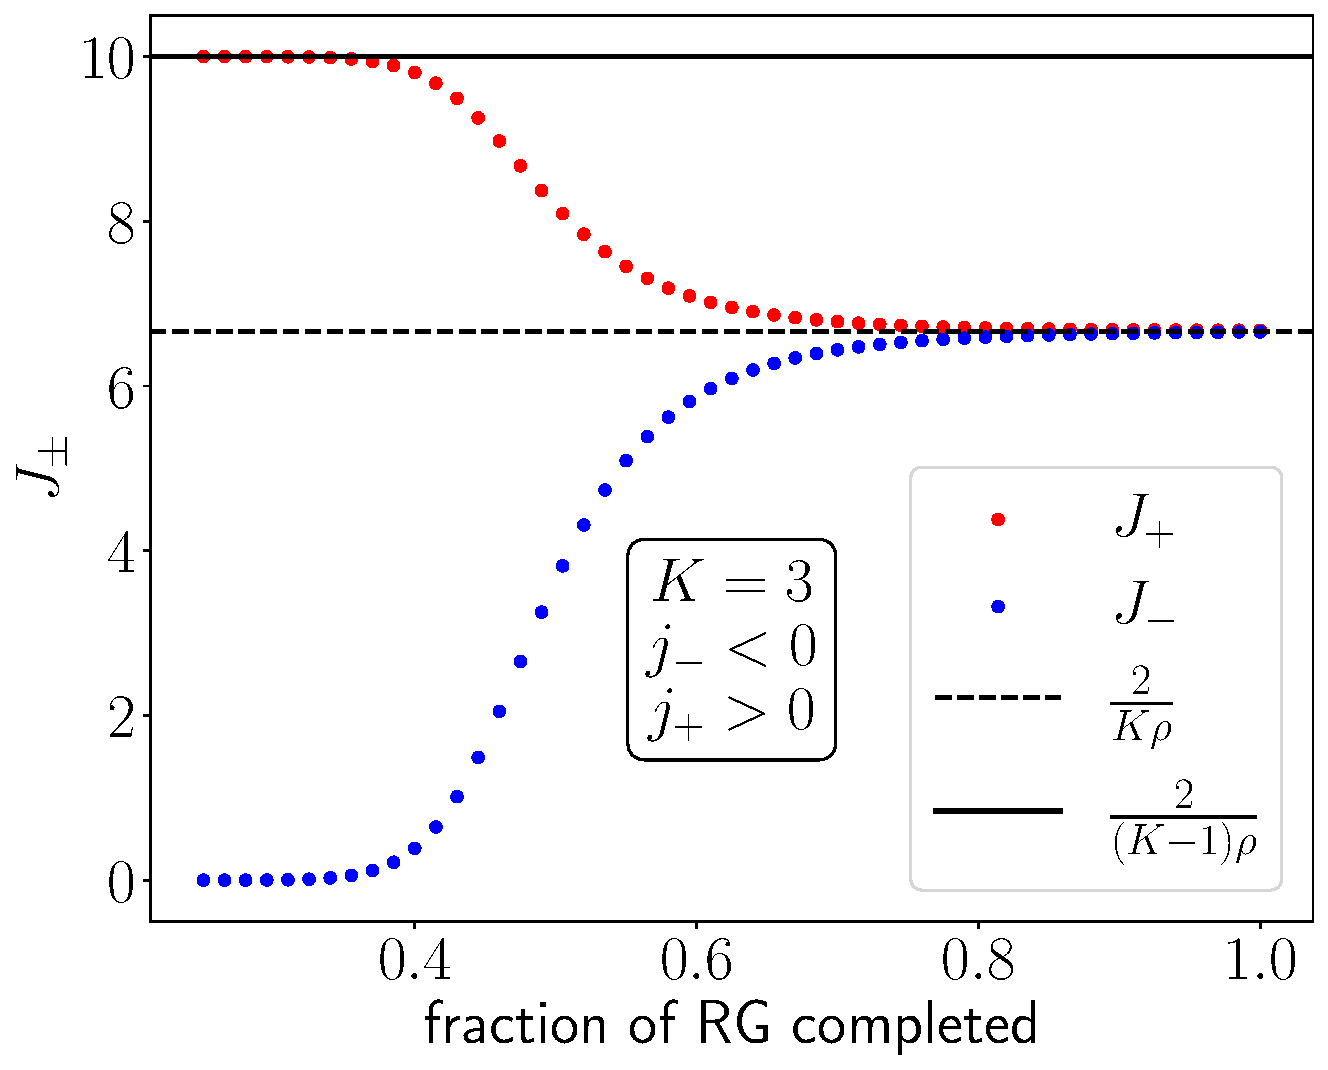
\includegraphics[width=0.32\textwidth]{../numerics/K to K-1.pdf}
	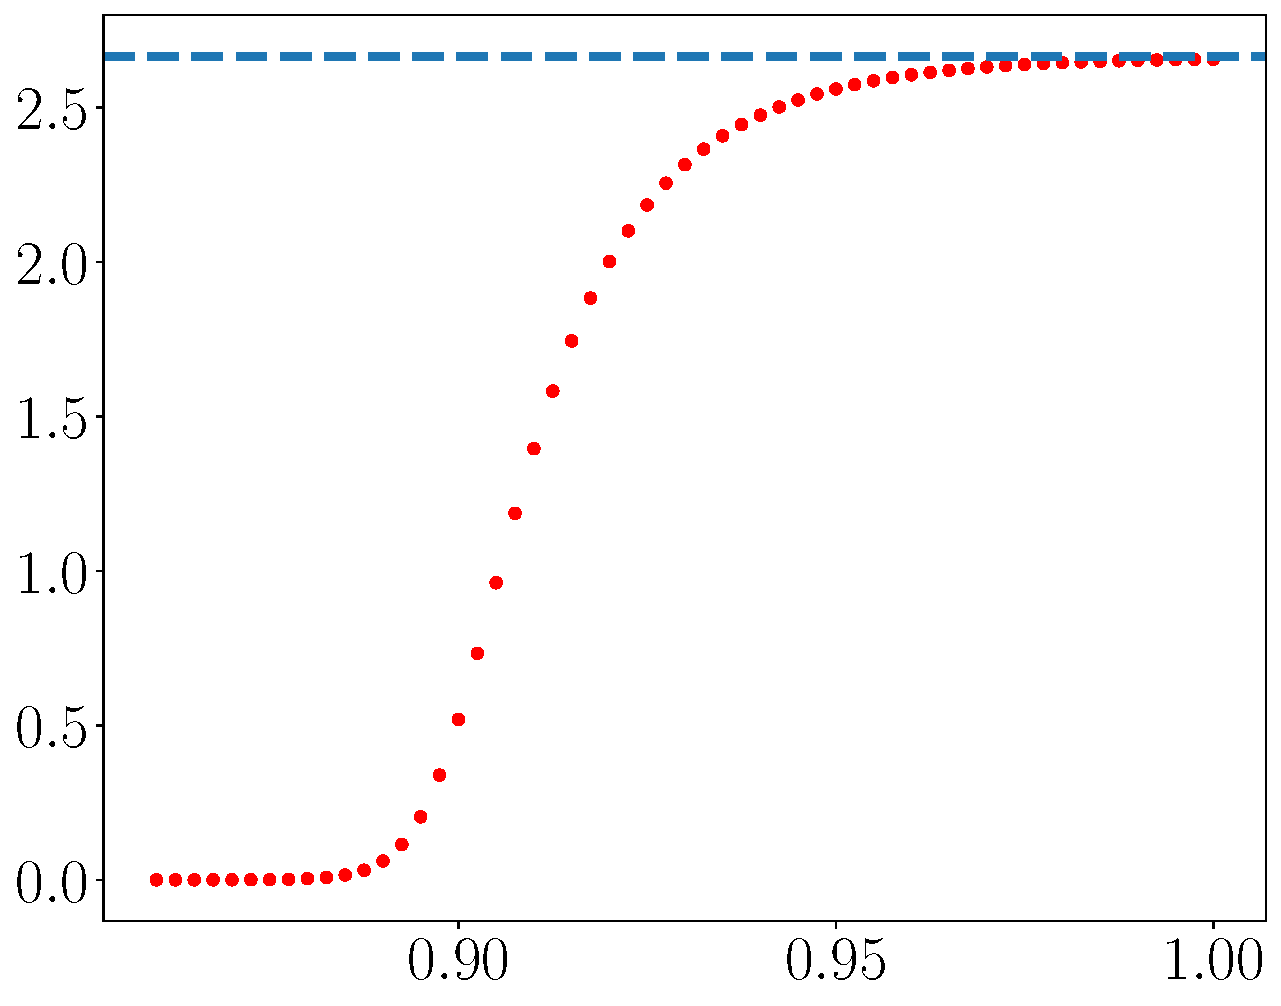
\includegraphics[width=0.32\textwidth]{../numerics/irr_Jp_K=3.pdf}
	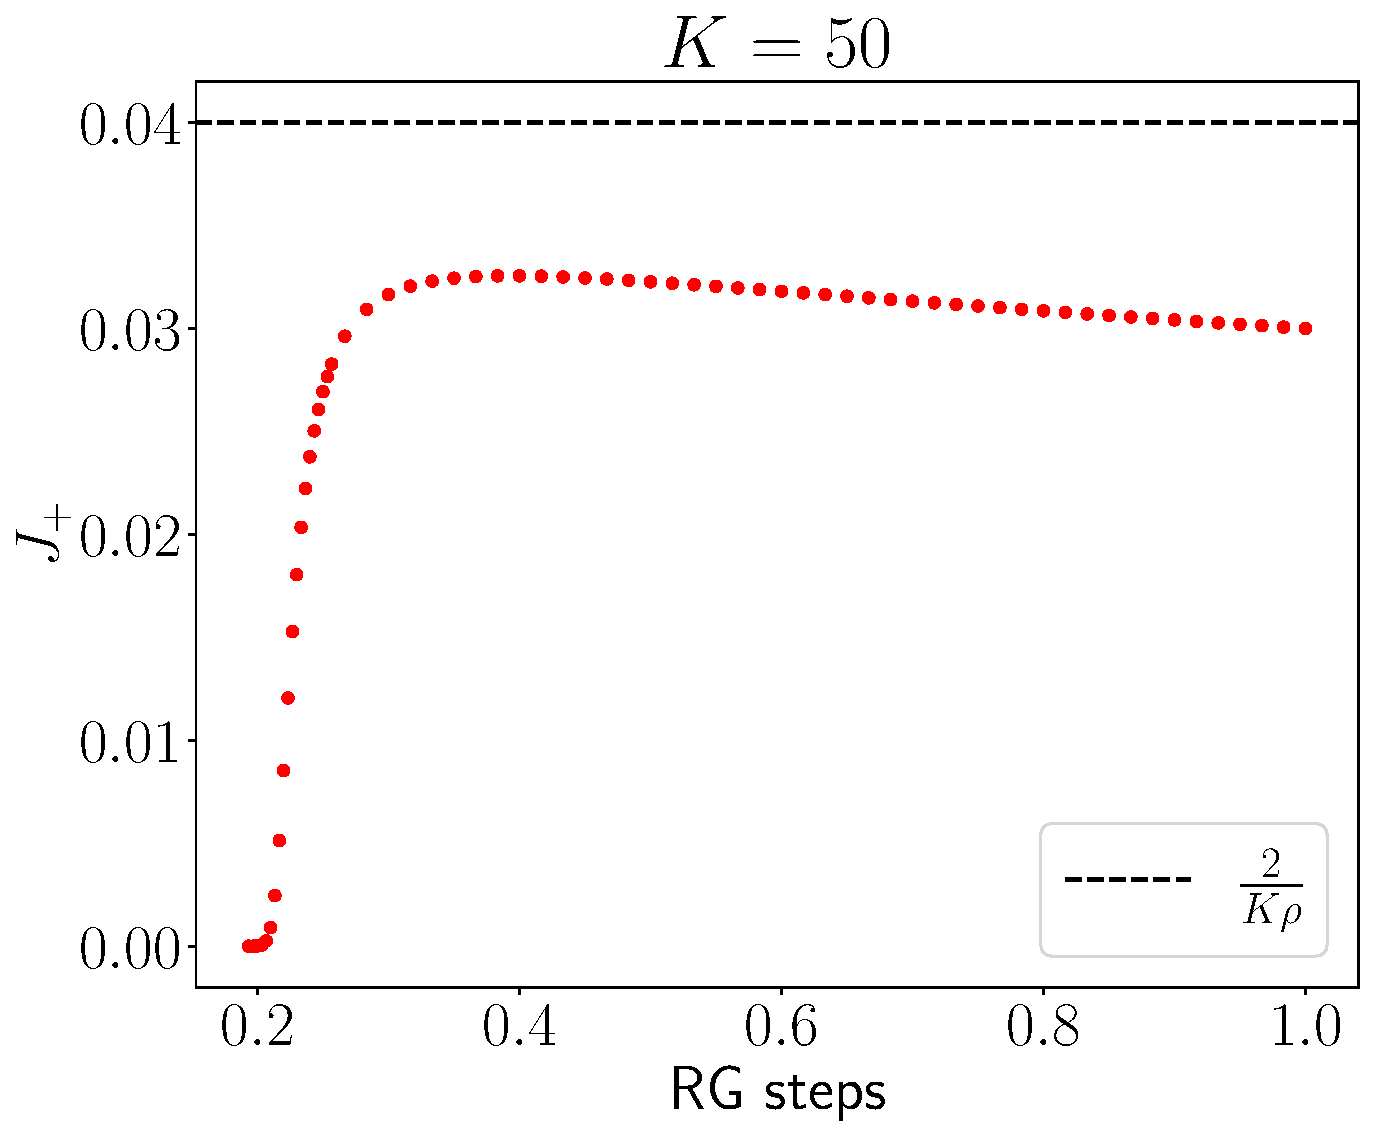
\includegraphics[width=0.32\textwidth]{../numerics/irr_Jp_K=50.pdf}
	\caption{left panel: Flow of \(J_\pm\) when \(j_< 0\) and \(J_+\). The smaller coupling \(J_-\) is irrelevant and switches off, while the other \(K-1\) couplings \(J_+\) flow to the \(K-1\) MCK fixed point. Middle and right panels: Flow of the couplings \(J_+\) when \(j_+ < 0\) when \(j_- > 0, j_+ < 0\), for two values of \(K\). In both cases, the smaller coupling \(J_+\) eventually dies out, leading to only one surviving coupling \(J^-\) which is relevant, and we are left with a single-channel Kondo model.}
	\label{K_to_K-1}
\end{figure*}

In the opposite regime \(j_- > 0, j_+ < 0\), \(\Delta j_+\) is negative. It has been checked numerically that \(J_+\) ultimately flows to zero in this regime (middle and right panels of fig. \ref{K_to_K-1}), and \(J_-\) remains relevant. Since there is no numerator fixed point in the relevant coupling \(J_-\) and because all other couplings are irrelevant, the equation for \(J_-\) is replaced by the single-channel Kondo coupling URG equation, and the low-energy physics is then of strong coupling.

\section{Conclusions}
\lipsum[1-5]


\acknowledgments
The authors thank P. Majumdar, A. Mitchell, S. Sen, S. Patra, M. Mahankali and R. K. Singh for several discussions and feedback. Anirban Mukherjee thanks the CSIR, Govt. of India and IISER Kolkata for funding through a research fellowship. Abhirup Mukherjee thanks IISER Kolkata for funding through a research fellowship. AM and SL thank JNCASR, Bangalore for hospitality at the inception of this work. NSV acknowledges funding from JNCASR and a SERB grant (EMR/2017/005398).

% \clearpage
\appendix
\section{Hamiltonian RG of spin-\(S\) impurity MCK Model}
\label{appendix_urg}
The Hamiltonian for the channel-isotropic MCK model is given in eq.~\ref{mc_ham}. As mentioned in the same section, the Hamiltonian \(H_{(j-1)}\) of the \((j-1)^\text{th}\) RG step is obtained from the Hamiltonian \(H_{(j)}\) of the preceding RG step by applying a unitary transformation \(U_{(j)}\): \(H_{(j-1)} = U_{(j)} H_{(j)} U^\dagger_{(j)}\). The unitary transformation is obtained in terms of the fermionic operator \(\eta_{(j)}\):
\begin{gather}
	U_{(j)} = \frac{1}{\sqrt 2}\left(1 + \eta_{(j)} - \eta_{(j)}^\dagger\right)~, \\
	\hat \omega_{(j)} = H_{(j-1)} - H^i_{(j)},~T_{(j)} \equiv \text{Tr}\left(H_{(j)}c_{j}\right)~,\\
	\eta^\dagger_{(j)} = \frac{1}{\hat \omega_{(j)} - \text{Tr}\left(H_{(j)} \hat n_{j}\right) } c^\dagger_{j} T_{(j)}~.
\end{gather}
The operator \(\hat \omega_{(j)}\) encodes the quantum fluctuation scales arising from the interplay of the kinetic energy terms and the interaction terms of the Hamiltonian.

The URG equation for the single-channel Kondo model \cite{kondo_urg} shows a stable strong-coupling fixed point. Ferromagnetic interactions are irrelevant. Strictly speaking, that RG equation already encodes, in principle, the multi-channel behaviour, through a modified \(\hat \omega\). To extract this information, we consider the strong-coupling fixed-point \(J \gg D\) as a fixed point and analyze its stability from the star graph perspective. For the exactly-screened case, the star graph decouples from the conduction bath, leaving behind a local Fermi liquid interaction on the first site. Similarly, in the under-screened regime, the ground state is composed of states where the impurity spin is only partially screened by the conduction channels. If a particular configuration of the bath-impurity system has the total conduction bath spin down, the impurity will have a residual up spin. This induces a ferromagnetic super-exchange coupling that is irrelevant under RG, so this fixed point is stable as well. 

We now come to the over-screened case, where there is a residual spin on the conduction channel site. The neighbouring electrons will now hop in with spins opposite to that of the impurity, so an antiferromagnetic interaction will be induced, and such an interaction is relevant under the RG. This shows that the over-screened regime cannot have a stable strong-coupling fixed point, and we need to search for an intermediate coupling fixed point. We therefore need the generator of the unitary transformation that incorporates third order scattering scatterings explicitly. We should take account of all possible processes that render the set of states \(\left\{\ket{\hat n_{q\beta}=1},\ket{\hat n_{q\beta}=0}\right\}\) diagonal. The higher order generator itself has two scattering processes, such that the entire renormalisation term \(c^\dagger_{q\beta} T \eta\) has in total three coherent processes. The complete generator upto third order can be written as
\begin{widetext}
\begin{equation}\begin{aligned}
	\eta = \frac{1}{\hat \omega - H_D}T^\dagger c \simeq \frac{1}{\omega^\prime - H_D}T^\dagger c + \frac{1}{\omega^\prime - H_D}H_X \frac{1}{\omega^\prime - H_D} T^\dagger c + \frac{1}{\omega^\prime - H_D} T^\dagger c \frac{1}{\omega^\prime - H_D} H_X
\end{aligned}\end{equation}
where \(H_X = J \sum_{k,k^\prime < \Lambda_j, \alpha,\alpha^\prime}\vec{S_d}\cdot\vec{s}_{\alpha \alpha^\prime}c^\dagger_{k\alpha}c_{k^\prime\alpha^\prime}\) is scattering between the entangled electrons. There are two third order terms in the above equation corresponding to the two possible sequences in which the processes can occur while keeping the total renormalisation \(c^\dagger_{q\beta}T \eta\) diagonal in \(q\beta\). The second order processes remain unchanged. The total renormalisation takes the form:
\begin{equation}
	\label{full_ren}
	\Delta H_{(j)} = \underbrace{c^\dagger T \frac{1}{\omega^\prime - H_D} T^\dagger c  + \left(c^\dagger \leftrightarrow c\right)}_{\Delta H^{(2)}_{(j)}} + \underbrace{c^\dagger T \frac{1}{\omega^\prime - H_D} H_X \frac{1}{\omega^\prime - H_D} T^\dagger c + c^\dagger T \frac{1}{\omega^\prime - H_D} T^\dagger c \frac{1}{\omega^\prime - H_D} H_X + \left(c^\dagger \leftrightarrow c\right)}_{\Delta H^{(3)}_{(j)}}
\end{equation}
\(\Delta H^{(2)}_{(j)}\) and \(\Delta H^{(3)}_{(j)}\) are the renormalisation arising from the the second and third order processes respectively.

It is easier to see the RG flow of the couplings if we write the Hamiltonian in terms of the eigenstates of \(S_d^z\). These eigenstates are defined by \(S_d^z\ket{m_d} = m_d\ket{m_d}, m_d \in \left[-S, S\right]\). In terms of these eigenstates, the Hamiltonian becomes
\begin{equation}\begin{aligned}
	\label{H_spin_S}
	\mathcal{H} = \sum_{k\sigma}\epsilon_{k}\tau_{k\sigma} + \sum_{m_d=-S}^S \sum_{kl,\atop{\sigma=\uparrow,\downarrow}} J^\sigma_{m_d} \ket{m_d}\bra{m_d} c^\dagger_{k \sigma}c_{l \sigma} + \sum_{kl} \sum_{m_d=-S}^{S-1} J^t_{m_d} \left(\ket{m_d+1}\bra{m_d} s^-_{kl}  + \text{h.c.}\right)
\end{aligned}\end{equation}
\end{widetext}
where \(k,l\) sum over the momentum states, \(\sigma\) sums over the spin indices, \(J^\sigma_m = \frac{1}{2} \sigma m J\) in the UV Hamiltonian, and \(J^t_{m} = J\frac{1}{2}\sqrt{S(S+1) - m(m+1)}\) is the coupling that connects \(\ket{m}\) and \(\ket{m+1}\). We first calculate \(\Delta H^{(2)}_{(j)}\). There will be two types of processes - those processes that start from an occupied state (particle sector) and those that start from a vacant state (hole sector). Due to particle hole symmetry of the Hamiltonian, they will be equal to each other and we will only calculate the particle sector contribution. 

In the particle sector, we have (\(\hat n_{q\beta}=1\)), so we will work at a negative energy  shell \(\epsilon_q = -D\). The renormalisation can schematically represented as \(H^I_0 \frac{1}{\omega - H^D_{q\beta}} H^I_1\). Both \(H^I_0\) and \(H^I_1\) have all three operators \(S_d^z, S_d^\pm\). We first consider specifically the case of spin-\(\frac{1}{2}\) impurity. Those terms that have identical operators on both sides can be ignored because \({S_d^z}^2 = \text{constant}\) and \({S^\pm}^2 = 0\). All the six terms that \textit{will} renormalise the Hamiltonian have a spin flip operator on at least one side of the Greens function. This means that in the denominator of the Greens function, \(S_d^z\) and \(s^z_{qq}\) have to be anti-parallel in order to produce a non-zero result for that term. This means we can identically replace \(S_d^z s^z_{qq} = -\frac{1}{4}\). Also, in the particle sector, the Greens function always has \(c_{q\beta}\) in front of it, so \(\epsilon_q \tau_{q\beta} = \frac{D}{2}\). The upshot of all this is that the denominator of all scattering processes for the spin-\(\frac{1}{2}\) impurity Hamiltonian will be \(\omega - \frac{D}{2} + \frac{J}{4}\).

We now come to the general case of spin-\(S\) impurity. The various terms that renormalise the Hamiltonian can be described in terms of the bath spin operators that come into them. For example, the term that has \(s^z\) on both sides of the intervening Greens function can be represented as \(z|z\). There are 7 such terms: \(z|z, \pm|\mp, z|\pm, \pm|z\). Each of these terms occur both in the particle and the hole sectors. We will demonstrate the calculation of two of these terms. The \(z|z\) \(+|-\) terms evaluate in the following manner.
\begin{widetext}
\begin{align}
	z|z: & \sum_{kk^\prime,m,\sigma} c^\dagger_{q \sigma} c_{k^\prime \sigma} \ket{m}\bra{m}\frac{{J^\sigma_m}^2}{\omega - \frac{D}{2} + \frac{J}{2}\sigma S_d^z}\ket{m}\bra{m} c^\dagger_{k \sigma}c_{q \sigma} = -\sum_{kk^\prime,m,\sigma}n_{q \sigma}\frac{{J^\sigma_m}^2 c^\dagger_{k \sigma}c_{k^\prime\sigma} \ket{m}\bra{m}}{\omega_{m, \sigma} - \frac{D}{2} + \frac{J}{2}\sigma m}\\
	+|-: & \sum_{kk^\prime,m} c^\dagger_{q \uparrow} c_{k^\prime \downarrow} \ket{m}\bra{m+1}\frac{{J^t_m}^2}{\omega - \frac{D}{2} + \frac{J}{2}S_d^z}\ket{m+1}\bra{m} c^\dagger_{k \downarrow}c_{q \uparrow} = -n_{q \uparrow}\sum_{kk^\prime,m}\frac{{J^t_m}^2 c^\dagger_{k \downarrow}c_{k^\prime\downarrow} \ket{m}\bra{m}}{\omega_{m+1, \uparrow} - \frac{D}{2} + \frac{J}{2}\left( m+1 \right) }
\end{align}
\end{widetext}
We similarly compute the rest of the terms. We again define \(\sum_q \hat n_{q\sigma} = n(D)\). To compare with the spin-\(\frac{1}{2}\) RG equations, we will transform the general spin-\(S\) \(\omega\) to the spin-\(\frac{1}{2}\) \( \omega\), using \(\omega_{m,\sigma} \to \omega - \frac{J}{2}\left(m\sigma - \frac{1}{2}\right)\).

The renormalisation in \(J^\sigma_m\) is
\begin{equation}\begin{aligned}
	\Delta J^\sigma_{m} = - n(D) \frac{\left( J^\sigma_m \right) ^2 + \left( J^t_{m-\frac{1+\sigma}{2}} \right) ^2}{\omega - \frac{D}{2} + \frac{J}{4}}~.
\end{aligned}\end{equation}
Here, we have defined \(J^t_m = 0\) for \( |m| > S\). Two relations can be obtained from this RG equation, the RG equations for the sum and difference of the couplings: \(J^\pm_m = \frac{1}{2}\left(J^\uparrow_m \pm J^\downarrow_m\right) \). The RG equation for the sum of the couplings is
\begin{equation}\begin{aligned}
	\Delta J^+_m = -n(D)\frac{\sum_\sigma \left( J^\sigma_m \right) ^2 + \sum_\sigma \left( J^t_{m-\frac{1+\sigma}{2}} \right) ^2}{2\left(\omega - \frac{D}{2} + \frac{J}{4}\right)}\\
	= -n(D)\frac{J^2}{4}\frac{S(S+1)}{\omega - \frac{D}{2} + \frac{J}{4}}
\end{aligned}\end{equation}
This is an \(m-\)independent piece, so it can be summed over to produce an impurity-independent potential scattering term, which we ignore. 

The second is the RG equation for the difference of the couplings:
\begin{equation}\begin{aligned}
	\Delta J^-_m = -n(D)\frac{1}{2}\frac{\left( J^t_{m-1} \right) ^2 - \left(J^t_{m}\right) ^2}{\omega - \frac{D}{2} + \frac{J}{4}} = -\frac{1}{4}\frac{n(D) m J^2}{\omega - \frac{D}{2} + \frac{J}{4}}
\end{aligned}\end{equation}
The usual \(J\) Kondo coupling is recovered through \(J = 2J^-_m/m\). Substituting this gives 
\begin{equation}\begin{aligned}
	\Delta_\text{p sector} J = -\frac{1}{2}n(D)\frac{J^2}{\omega - \frac{D}{2} + \frac{J}{4}}
\end{aligned}\end{equation}

We can also obtain the RG equation for \(J\) from the transverse renormalisation:
\begin{equation}\begin{aligned}
	\Delta J^t_m &= - \frac{n(D)J^t_m \left( J^\downarrow_m + J^\uparrow_{m+1} \right) }{\omega - \frac{D}{2} + \frac{J}{4}} = -\frac{1}{2}\frac{n(D)J^t_m J}{\omega - \frac{D}{2} + \frac{J}{4}}
\end{aligned}\end{equation}
Since \(J^t_m \propto J\), we have
\begin{equation}\begin{aligned}
	\Delta J_\text{p sector} &= -\frac{1}{2}\frac{n(D)J^2}{\omega - \frac{D}{2} + \frac{J}{4}}
\end{aligned}\end{equation}
The total renormalisation from both particle and hole sectors, at this order, is
\begin{equation}\begin{aligned}
	\Delta J^{(2)} &= -\frac{n(D)J^2}{\omega - \frac{D}{2} + \frac{J}{4}}
\end{aligned}\end{equation}

We now come to the third order renormalisation.
Following eq.~\ref{full_ren}, the next order renormalisation is
\begin{equation}\begin{aligned}
	\label{psector_3rd_ren}
	\Delta H^{(3)}_j = c^\dagger T \frac{1}{\omega^\prime - H_D} H_X \frac{1}{\omega^\prime - H_D} T^\dagger c \\
	+ c^\dagger T \frac{1}{\omega^\prime - H_D} T^\dagger c \frac{1}{\omega^\prime - H_D} H_X
\end{aligned}\end{equation}
The first term will be of the form
\begin{widetext}
\begin{equation}\begin{aligned}
	\sum_{q,k,l_1} c^\dagger_{q\beta, l_1}c_{k \alpha, l_1}\ket{m_1}\bra{m_2} \frac{1}{\omega - \frac{D}{2} - \frac{\epsilon_k}{2} + \frac{\beta J}{4}S_d^z} \ket{m_2} c^\dagger_{k_1 \sigma_1, l_2}c_{k_2 \sigma_2,l_2} \bra{m_3}\frac{1}{\omega - \frac{D}{2} - \frac{\epsilon_k}{2} + \frac{\beta J}{4}S_d^z}\ket{m_3}\bra{m_4}c^\dagger_{k\alpha, l_1}c_{q\beta, l_1}
\end{aligned}\end{equation}
\end{widetext}
We have not bothered to write all the summations and the couplings correctly, because we will only simplify the denominator here. Evaluating the inner products gives
\begin{equation}\begin{aligned}
	\sum_{qk,l_1} \frac{\ket{m_1}\bra{m_4}c^\dagger_{q\beta}c_{k \alpha}c^\dagger_{k_1 \sigma_1, l_2}}{\omega_{m_2,\beta} - \frac{D}{2} - \frac{\epsilon_k}{2} + \frac{\beta J m_2}{4}}  \frac{c_{k_2 \sigma_2,l_2}c^\dagger_{k\alpha}c_{q\beta}}{\omega_{m_3,\beta} - \frac{D}{2} - \frac{\epsilon_k}{2} + \frac{\beta J m_3}{4}}
\end{aligned}\end{equation}
We again use \(\omega_{m,\sigma} \to \omega - \frac{J}{2}\left(m\sigma - \frac{1}{2}\right)\).
\begin{equation}\begin{aligned}
	\ket{m_1}\bra{m_4}c^\dagger_{k_1 \sigma_1, l_2}c_{k_2 \sigma_2,l_2}\sum_{qk,l_1} \frac{\hat n_{q\beta}\left(1 - \hat n_{k\alpha}\right)}{\left(\omega - \frac{D}{2} - \frac{\epsilon_k}{2} + \frac{J}{4}\right)^2}
\end{aligned}\end{equation}
We define \(\sum_q \hat n_{q\beta} = n(D)\). Performing the sums over \(k\) and \(l_1\) gives
\begin{equation}\begin{aligned}
	-\frac{1}{2}\ket{m_1}\bra{m_4}c^\dagger_{k_1 \sigma_1, l_2}c_{k_2 \sigma_2,l_2} \frac{\rho n(D) K}{\omega - \frac{D}{2} + \frac{J}{4}}
\end{aligned}\end{equation}
\(\rho\) is the density of states which we have taken to be constant. Reinstating the complete summation and the couplings gives
\begin{equation}\begin{aligned}
	\label{first_group}
	-\frac{1}{2}\frac{\rho n(D) K}{\omega - \frac{D}{2} + \frac{J}{4}}\sum_{m_1,m_4,k_1,k_2,\atop{l_2,\sigma_1\sigma_2}}\lambda_{1}\lambda_{2}\lambda_{3}\ket{m_1}\bra{m_4}c^\dagger_{k_1 \sigma_1, l_2}c_{k_2 \sigma_2,l_2}
\end{aligned}\end{equation}
There is no sum over \(m_2\) and \(m_3\) because they are constrained by \(m_1\) and \(m_4\) respectively. \(\lambda_i\) represent the couplings present at the three interaction vertices. \(k_{1,2}\) sum over the momenta, \(\sigma_{1,2}\) sum over the spin indices and \(l_2\) sums over the channels.

The second term in eq.~\ref{psector_3rd_ren} can be evaluated in an almost identical fashion. The integral here be negative of the first term, because of an exchange in the scattering processes.
\begin{equation}\begin{aligned}
	\label{second_group}
	\frac{1}{2}\frac{\rho n(D) K}{\omega - \frac{D}{2} + \frac{J}{4}}\sum_{m_1,m_4,k_1,k_2,\atop{l_2,\sigma_1\sigma_2}}\lambda_{1}\lambda_{3}\lambda_{2}\ket{m_1}\bra{m_4}c^\dagger_{k_1 \sigma_1, l_2}c_{k_2 \sigma_2,l_2}
\end{aligned}\end{equation}

The first group of terms (those that appear in \ref{first_group}) in the particle sector can be represented as \(a|b^\prime|c\), where \(a,b,c \in \left\{z,+,-\right\} \) and represent the operator for the conduction electrons in the three ceonnected processes. The \(\prime\) on \(b\) indicates that it is the state of the electrons \textit{not being decoupled}. The second group of terms (those that appear in \ref{second_group}) are therefore represented as \(a|b|c^\prime\), because in this group, the interaction \(H_X\) between the electrons that are not being decoupled occur at the very end.
We will only calculate the terms in the particle sector, the ones in hole sector will be equal to these because of particle-hole symmetry. The full list of terms is: 
$z|z^\prime|z\quad$
$z|z|z^\prime\quad$
$-|z^\prime|+\quad$
$-|+|z^\prime\quad$
$+|z^\prime|-\quad$
$+|-|z^\prime\quad$
$ z|+^\prime|z\quad$
$z|-^\prime|z\quad$
$+|+^\prime|-\quad$
$-|+^\prime|+\quad$
$z|z|+^\prime\quad$
$z|z|-^\prime\quad$
$ +|-|+^\prime\quad$
$+|-|-^\prime\quad$
$-|+|+^\prime\quad$
$z|z^\prime|z\quad$
$z|z|z^\prime\quad$
$-|z^\prime|+\quad$
$ -|+|z^\prime\quad$
$+|z^\prime|-\quad$
$+|-|z^\prime\quad$
$z|+^\prime|z\quad$
$z|-^\prime|z\quad$
$+|+^\prime|-\quad$
$-|+^\prime|+\quad$
$z|z|+^\prime\quad$
$z|z|-^\prime\quad$
$+|-|+^\prime\quad$
$+|-|-^\prime\quad$
$-|+|+^\prime\quad$
.

The total renormalisation in  \(J^\sigma_m\) is
\begin{widetext}
\begin{equation}\begin{aligned}
	\Delta J^\sigma_m = \frac{1}{2}\frac{\rho n(D) K}{\omega - \frac{D}{2} + \frac{J}{4}}\left[\left( J^t_{m-1} \right)^2 J^\sigma_m + \left( J^t_m \right)^2 J^\sigma_m - \left( J^t_{m-1} \right)^2 J^\sigma_{m-1} - \left(J^t_m\right)^2 J^\sigma_{m+1} \right] = \frac{1}{2}\frac{\rho n(D) K}{\omega - \frac{D}{2} + \frac{J}{4}}J^3 m \sigma
\end{aligned}\end{equation}
Since we had defined \(J^\sigma_m \equiv \frac{1}{2}J m \sigma\), we have \(\Delta J = \frac{2}{m\sigma}\Delta J^\sigma_m\), and we get \(\Delta_\text{p sector} J = \frac{1}{4}\frac{\rho n(D) K}{\omega - \frac{D}{2} + \frac{J}{4}}J^3\).
Combining with the hole sector renormalisation, we get
\begin{equation}\begin{aligned}
	\Delta J^{(3)} = \frac{1}{2}\frac{\rho n(D) K}{\omega - \frac{D}{2} + \frac{J}{4}}J^3
\end{aligned}\end{equation}
The total renormalisation in \(J\) after combining all orders is
\begin{equation}\begin{aligned}
	\Delta J = -\frac{n(D) J^2}{\omega - \frac{D}{2} + \frac{J}{4}} + \frac{1}{2}\frac{\rho n(D) K}{\omega - \frac{D}{2} + \frac{J}{4}}J^3
\end{aligned}\end{equation}
\end{widetext}


\bibliography{mscript_mck}
\end{document}
